\documentclass[a4paper,12pt,headsepline]{scrartcl}

%\part{title}
\usepackage[utf8]{inputenc}
\usepackage{graphicx}
\usepackage{caption,subcaption}
\usepackage[english]{babel}
\usepackage[T1]{fontenc}
\usepackage{proof}
\usepackage{hyperref}
%\usepackage[hyphens,obeyspaces,spaces]{url}
\usepackage{fancybox}
\usepackage{amssymb,amsmath,amsthm}
\usepackage{textcomp}
\usepackage{gensymb}
\usepackage[linesnumbered,ruled,vlined,norelsize]{algorithm2e}
\usepackage{algpseudocode}
% \usepackage[bookmarksnumbered,hyperfootnotes=false]{hyperref} % ,pdftitle={\titleDocument}
\usepackage{color}
\usepackage{float}
\usepackage[backend=biber]{biblatex}
\bibliography{Bibliography} % bib file name

\usepackage{geometry}
\geometry{left=3.5cm, right=2cm, top=2.5cm, bottom=2cm}


%test
\usepackage[backend=biber]{biblatex}
\usepackage{filecontents}

% \addbibresource{ref.bib}

\restylefloat{figure}

% Makros
\newenvironment{sketch}{\begin{proof}[Proof (Sketch)]}{\end{proof}}
\newtheorem{theorem}{Theorem}
\newtheorem{assumption}{Assumption}
\newtheorem{lemma}{Lemma}
\newtheorem{remark}{Remark}
\newtheorem{definition}{Definition}
\newtheorem{corollary}{Corollary}
\newtheorem{observation}{Observation}
\newtheorem{fact}{Fact}
\newcommand{\comment}[1]
{
	\begin{quotation}
		\textcolor{blue}{\underline{Edit:} #1}
	\end{quotation}
}
\newcommand{\TODO}[1]
{
	\begin{quotation}
		\textcolor{red}{\underline{TODO:} #1}
	\end{quotation}
}

\newcommand{\Kommentar}[1]
{
	\begin{quotation}
		\textcolor{blue}{\underline{Kommentar:} #1}
	\end{quotation}
}
% Symbols
\newcommand{\N}{\ensuremath{\mathbb{N}}}
\newcommand{\UL}{\texttt{UL}}

% neue Kopfzeilen mit fancypaket
\usepackage{fancyhdr} %Paket laden
\pagestyle{fancy} %eigener Seitenstil
\fancyhf{} %alle Kopf- und Fußzeilenfelder bereinigen
\fancyhead[L]{\nouppercase{\leftmark}} %Kopfzeile links
\fancyhead[C]{} %zentrierte Kopfzeile
\fancyhead[R]{\thepage} %Kopfzeile rechts
\renewcommand{\headrulewidth}{0.4pt} %obere Trennlinie
%\fancyfoot[C]{\thepage} %Seitennummer
%\renewcommand{\footrulewidth}{0.4pt} %untere Trennlinie

\frenchspacing
\makeindex

% Pseudocode für Java
%\usepackage{listings}
%\lstset{numbers=left, numberstyle=\tiny, numbersep=5pt, keywordstyle=\color{black}\bfseries, stringstyle=\ttfamily,showstringspaces=false,basicstyle=\footnotesize,captionpos=b}
%\lstset{language=java}

% Disable single lines at the start of a paragraph (Schusterjungen)
\clubpenalty = 10000
% Disable single lines at the end of a paragraph (Hurenkinder)
\widowpenalty = 10000
\displaywidowpenalty = 10000



\begin{document}
% das Papierformat zuerst
%\documentclass[a4paper, 11pt]{article}

% deutsche Silbentrennung
%\usepackage[ngerman]{babel}

% wegen deutschen Umlauten
%\usepackage[ansinew]{inputenc}

% hier beginnt das Dokument
%\begin{document}


\thispagestyle{empty}

%\begin{figure}[t]
% \centering
% \includegraphics[width=0.6\textwidth]{abb/logo1}
%~~~~~~~~~~
% \includegraphics[width=0.3\textwidth]{abb/logo2}
%\end{figure}


\begin{verbatim}
	
	
\end{verbatim}

\begin{center}
	\Large{Eberhard Karls Universität Tübingen}\\
	\small Wilhelm Schickard Institut Tübingen\\
\end{center}


\begin{center}
	\Large{Fachbereich Informatik}
\end{center}
\begin{verbatim}
	
	
	
	
\end{verbatim}
\begin{center}
	%\doublespacing
	\textbf{\LARGE{Minimizing the edge length ratio of planar poly-line graph drawings}}\\
	%\singlespacing
	\begin{verbatim}
		
	\end{verbatim}
	\textbf{{Arbeitsbereich Algorithmik}}
\end{center}
\begin{verbatim}
	
\end{verbatim}
\begin{center}
	
\end{center}
\begin{verbatim}
	
\end{verbatim}
\begin{center}
	\textbf{Forschungsprojekt SS21}
\end{center}
\begin{verbatim}
	
	
	
	
	
	
\end{verbatim}
\begin{flushleft}
	\begin{tabular}{llll}
		\textbf{Autor:} & & Benjamin Ulvi \c Coban & \\
		& & MatNr. 3526251 & \\
		& & \\
		\textbf{Version vom:} & & \today &\\
		& & \\
		\textbf{Betreuer:} & & Prof. Dr. Michael Kaufmann &\\
	\end{tabular}
\end{flushleft}
\section{Introduction}
The topic of visualization of information relationships occur in various areas of work. Examples of the fields include circuit design, architecture, web science, social sciences, biology, geography, information security and software engineering. The relationships of various information is formalized \textcolor{red}{What is an undirected planar graph, what are bends, grid, poly-line, edge-length}

\section{Preliminaries}
As otherwise mentioned, a \textit{graph} $G=(V_G,E_G)$ is a tuple consisting of two sets - the set of vertices and the set of edges. An \textit{edge} $e = (v,w), v,w \in V_G$ is a tuple and describes a connectivity relation between two vertices. Unless otherwise mentioned, the graphs are \textit{undirected}. It means that the edge $(u,v)$ is identical to the edge $(v,u)$,$u,v\in V_G$. A \textit{face} is a maximal open region of the plane bounded by edges. The degree of the graph is the amount of edges attached to it. A graph $G'$ is called a supergraph of $G$ iff $V_{G}\subseteq V_{G'}$ and $E_{G}\subseteq E_{G'}$. 
\bigskip\\
 A \textit{drawing} $\Gamma$ of a graph $G$ is a function, where each vertex is mapped on a unique point $\Gamma(v)$ in the plane and each edge is mapped on an open Jordan curve $\Gamma(e)$ ending in its vertices. A graph is \textit{planar} if and only if there exists a crossing-free representation in the plane. $G$ is maximal planar iff any further edge insertion violates the planarity property. A $k\times k$ grid is an undirected graph consisting of $k$ rows and $k$ columns of vertices. A vertex in the $i$-th row and $j$-th column is denoted as $(i,j)$.\\
 A straight line drawing on a grid of size $k\times k$ is a drawing where every vertex has its unique row and column value and every edge is drawn as a straight line. In a polyline drawing, each edge is represented by a non-empty sequence of line segments ($e = (e_1,e_2,...)$), where two consecutive line segments intersect in a unique point, a bend. Every bend lies, like the vertices, on a unique grid point.\bigskip\\
 To measure the length, the euclidian distance of a line segment is introduced as a metric. It is defined as the square root of the sum of the quadratic difference of row and column. The unit length, \UL in short, is defined as the distance between two consecutive points on the grid with either the same row or column value.\bigskip\\
 A path is a sequence of edges. A cycle is a path, so that the starting vertex and the ending vertex are identical. A tree is an acyclic graph. A graph is called connected if there is a path from every vertex to every other vertex of $G$. A $k$-ary tree is a graph where either every vertex has exactly $k$ children and one parent or is of degree 1. These are called leaves. The root of a tree is a vertex with no parent. The height of a tree is defined as the length of the longest path starting from the root. A tree is called complete, when all leaves have the same height and no further vertices can be inserted without increasing the maximum height.\bigskip\\
 A 2-terminal series-parallel graph with terminals $s,t$ is a recursively defined graph with one of the following three rules:
 \begin{enumerate}
 	\item An edge $(s,t)$ is a 2-terminal series-parallel graph
 	\item If $G_i, i = 1,2$, is a 2-terminal series-parallel graph with terminals $s_i,t_i$, then in the serial composition $t_1$ is identified with $s_2$ to obtain a 2-terminal series-parallel graph with $s_1,t_2$ as terminals
 	\item If $G_i, i=1,...,k$, is a 2-terminal series-parallel graph with terminals $s_i,t_i$, then in a parallel composition we identify all $s_i$ into one terminal $s$ and all $t_i$ into the other terminal $t$ and the result is a 2-terminal series-parallel graph with terminals $s,t$.
 \end{enumerate}
A series-parallel graph, SP-graph in short, is a graph for which every biconnected component is a 2-terminal series-parallel graph. A SP-graph is maximal if no edge can be added so while maintaining a SP-graph.\bigskip\\
A 2-tree is a recursively defined graph with at least three vertices. If $n = 3$, then the 2-tree is the $K_3$. If $n>3$, then start with a $K_3$ and every vertex added is adjacent to exactly two adjacend neighbours, forming a 3-clique. The class of 2-trees correspond to the class of maximal SP-graphs.~~[\cite{DBLP:journals/dcg/Biedl11}, Preliminaries], [\cite{DBLP:journals/jgaa/MondalNRA11}, Preliminaries], [\cite{DBLP:books/daglib/0023376}]

\section{The Problem}

% Copied from te symposium section
\subsection{The Symposium Challenge}
There has been recent attention to the edge-length ratio of a planar drawing, which describes the ratio between the lengths of the longest edge and the shortest edge in a drawing. 
\newline This year, the main topic addresses an optimization problem, namely the minimization of the edge-length ratio of poly-line drawings of planar, undirected graphs on a fixed grid. For a poly-line edge, the edge-length is the sum of the line segment lengths.
\bigbreak The input consists of a JSON file with the following entries:
\begin{description}
	\item[nodes] Every node has an unique ID value between 0 and the amount of nodes - 1, a value for the $x$ and $y$ coordinate each, delimited by the width and height
	\item[edges] Every edge has an ID for source and destination each and an optional list of bend points, specified in $x$ and $y$ coordinate
	\item[width (optional)] The maximum $x$-coordinate of the grid. If unspecified, the width is set to 1,000,000.
	\item[height (optional)] The maximum $y$ coordinate of the grid. If unspecified, the height is set to 1,000,000.
	\item[bends] The maximum number of bends allowed per edge
\end{description}
The results of the optimization are also JSON files. The planarity of the graph shall be preserved and the poly-line edge-length ratio minimized by relocation of the nodes.
\bigbreak For the teams participating with their own tools, an embedding might not be given with the input. For the participants working manually, an embedding is already given beforehand.
\cite{GDContest}
\subsection{Formalization Of The Problem}
\subsubsection{The edge-length ratio}
Let $\Omega_G$ be a given planar poly-line drawing. The length of an edge of $e$ is defined as the sum of $k+1$ line segments, induced by $k$ bends. $l_{\max}$ is the length of the longest edge in $\Omega_G$, $l_{\min}$ is the length of the shortest edge in $\Omega_G$. The edge-length ratio $r$ is defined as:
\begin{align}
	r = \frac{l_{\max}}{l_{\min}} 
\end{align}
It trivially holds, that $r\geq1$. $r$ is said to be optimal if $r=1$. Then, all the edges in a drawing are of the same length.
\subsubsection{Upper and lower bounds of the ratio}
A straight-line drawing $\Gamma_G$ is drawn with zero bends. There are multiple straight-line drawing algorithms which produce a drawing of area $\mathcal{O}(n)\times\mathcal{O}(n)$. The area consumption of a straight-line drawing directly induces the bounds for the ratio. Let $k\times k$ be the grid $\Gamma_G$ is drawn on, $k\in \mathcal{O}(n)$. The maximal length of a straight line is bound by $\sqrt{2}k$, from one corner of the grid to the diagonal opposing one, while the minimal length a straight line can inherit values obviously 1. The ratio therefore values $\sqrt{2}k$ in the worst case.\\
This automatically gives an upper bound for any poly-line drawing $\Omega_G$ since a straight-line drawing can be seen as a poly-line drawing with 0 bends. Bends will be included in a straight-line drawing to lengthen the shorter edges while the longest edge will be untouched.
\subsubsection{A small example - a triangle}
This example will illustrate the issue of finding a drawing with an optimal edge-length ratio. Consider $K_3$, the complete graph with three vertices. $K_3$ has got one outerface and one inner face, in shape of a triangle. In order to find a drawing of $K_3$ with an optimal ratio, we will see that one bend per edge is mandatory.\\
A triangle with straight-lines as edges with length $l$ will have a height of $\frac{\sqrt{3}}{2}l$ in order to be optimal regarding the ratio. Unfortunately, $\sqrt{3}$ is not a rational number. There do not exist two integers in order to express $\sqrt{3}$ as a fraction. As a consequence, there does not exist any combination of coordinates on a grid in order to draw the $K_3$ without any bends and an optimal ratio.
	\begin{figure}[H]
	\centering
	\begin{subfigure}{0.6\linewidth}
		\centering
		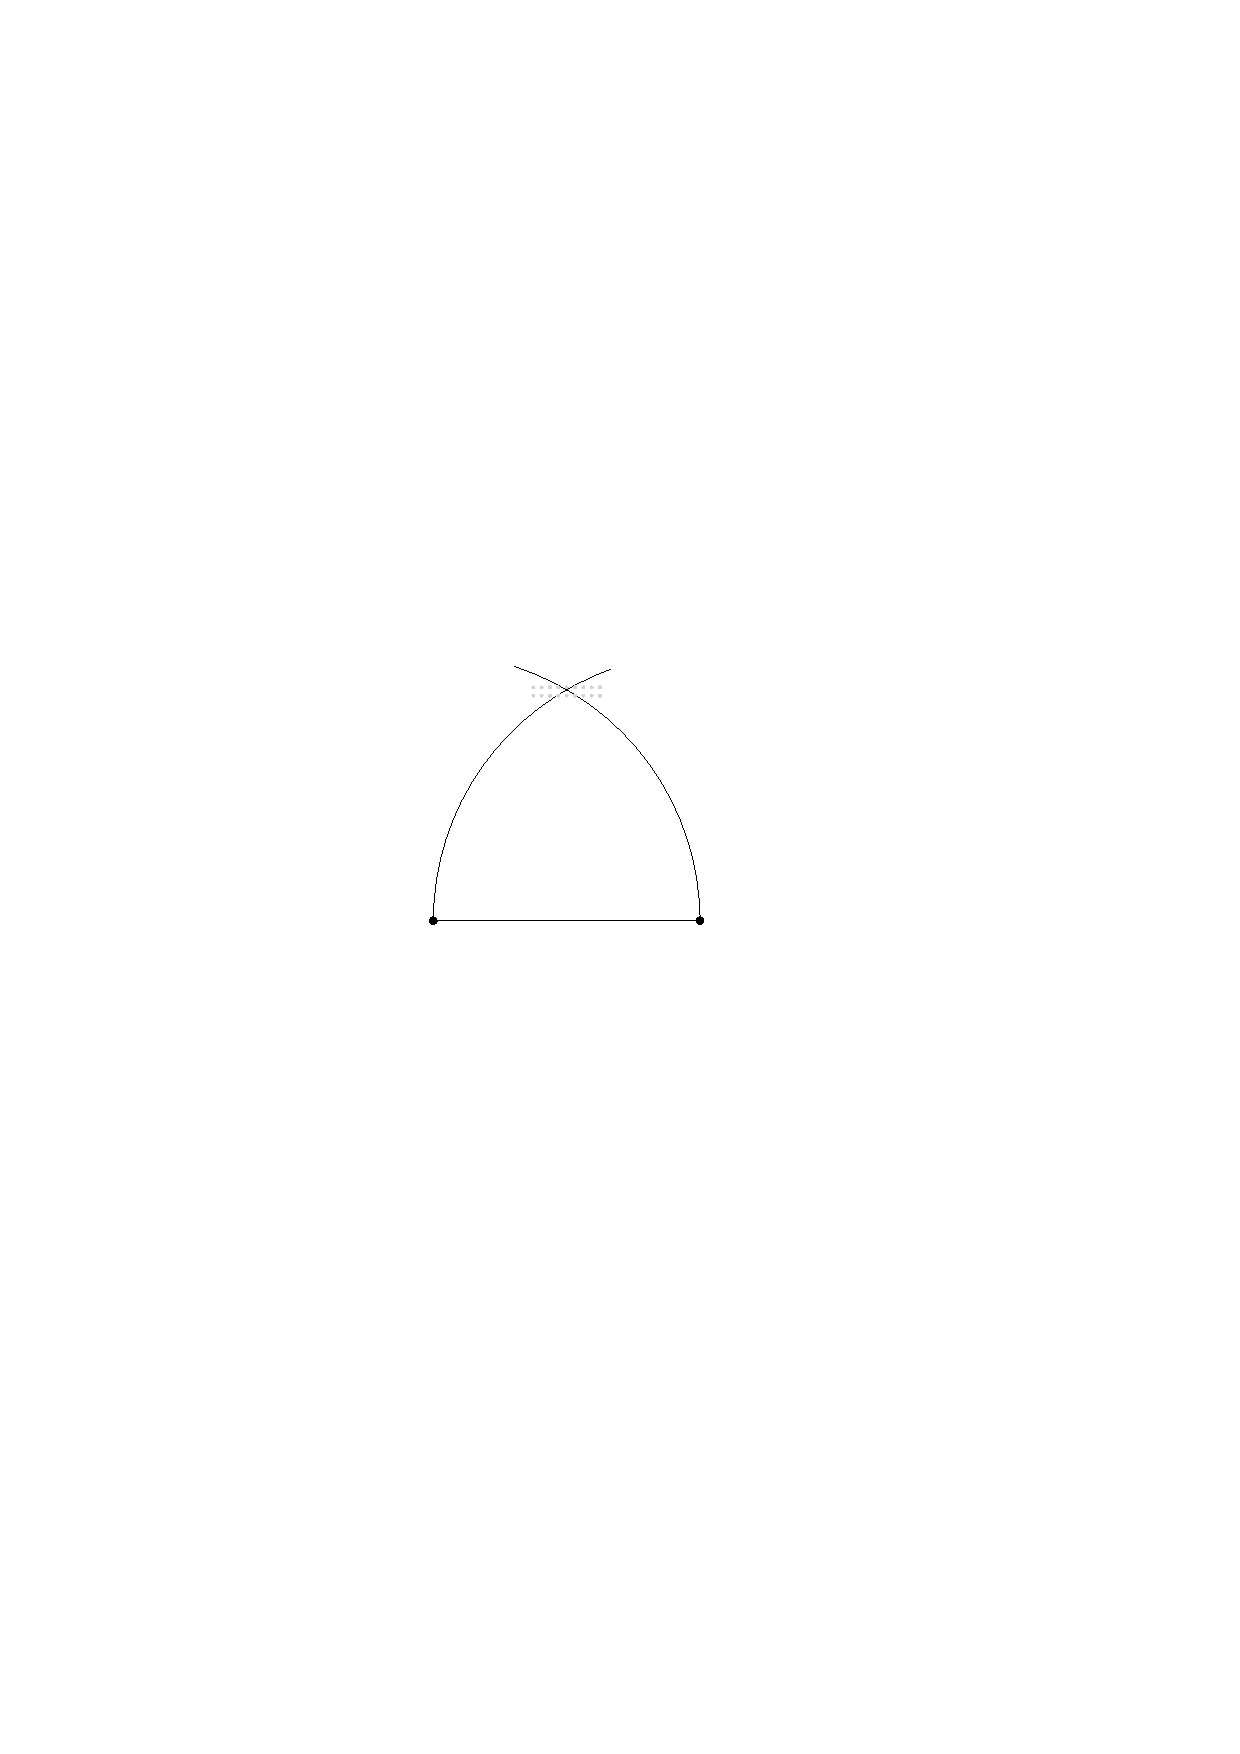
\includegraphics[width=0.7\textwidth,page=1]{drawings/small_example.pdf}
	\end{subfigure}
	\caption{There is no grid point for an optimal drawing without any bends}
\end{figure}

But, when introducing one bend per edge, there exists a drawing with an optimal ratio. 
\begin{figure}[H]
	\centering
	\begin{subfigure}{0.6\linewidth}
		\centering
		\includegraphics[width=0.7\textwidth,page=2]{drawings/small_example.pdf}
	\end{subfigure}
	\caption{With one bend, $K_3$ admits an optimal drawing}
\end{figure}
Allowing bends will help minimizing the ratio of a drawing. 
\section{Maximal planar graphs}
This section will demonstrate a postprocessing approach for an already given straight-line drawing of a maximal planar graph $G$, namely $\Gamma_G$, in order to minimize the edge-length ratio of planar graphs.\\
The main idea is to elongate the shortest edge as long as possible while still maintaining planarity. Obviously, the longest edge of $\Gamma_G$ will not be altered at all. The small length edges may be enclosed by small area faces which proves to be a challenge for a required elongation. In order to overcome this hurdle, the grid will be refined as much as is necessary. On the one hand, this increases the total area usage of the new drawing $\Gamma'_G$, but will provide sufficient area for any small length edge elongation on the other hand.\\
After the grid refinement, every inner face of $G$ will be subdivided evenly. For every face, a new vertex will be inserted which is adjacent to the vertices defining the face. This will extend $G$ to the supergraph $G'$. In the further process, the inserted edges and vertices serve as a guideline for the edge elongations.\\
Then, every straight line edge of $G$ that is smaller than the longest edge will be elongated using a linear amount of bends, altering the straight-line drawing to a poly-line drawing. The line segments will stay in the respective adjacent faces defined by $G'$. The reader will observe that the amount of bends and the factor of grid refinement will play along and the edge-length ratio will become a constant.


% Initial situation

\subsection{Initial situation}
At the beginning, a given straight-line drawing $\Gamma_G$ of a planar graph $G$ is given. We choose the drawing algorithm by Schnyder. The area consumption values $(n-1)\times(n-1)$ in the worst case \cite{Schnyder}.
When considering maximal planar graphs, the following fact describes the shape of every face of $G$.
\begin{fact}\label{fact:maximal-triangle}
\end{fact}
In a maximal planar graph $G$, every face is a triangle. Otherwise, $G$ is not maximal planar.
\begin{proof}[Proof by contradiction]
	Let $f$ be a face of $G$ defined by $k > 3$ vertices. Then, it is possible to insert at least one more edge into $f$, contradicting the maximal planarity of $G$.
\end{proof}

\bigskip
Regarding area consumption, the smallest possible face in $\Gamma_G$ is a triangle with two edges of \UL. If these smallest-area faces are adjacent to an edge, then there is no bend point on the grid availiable for further elongation. Each triangle consumes area of $\frac{1}{2}\UL^2$ and the length of $e$ cannot be increased.
\begin{figure}[H]
	\centering
	\begin{subfigure}{0.3\linewidth}
		\centering
		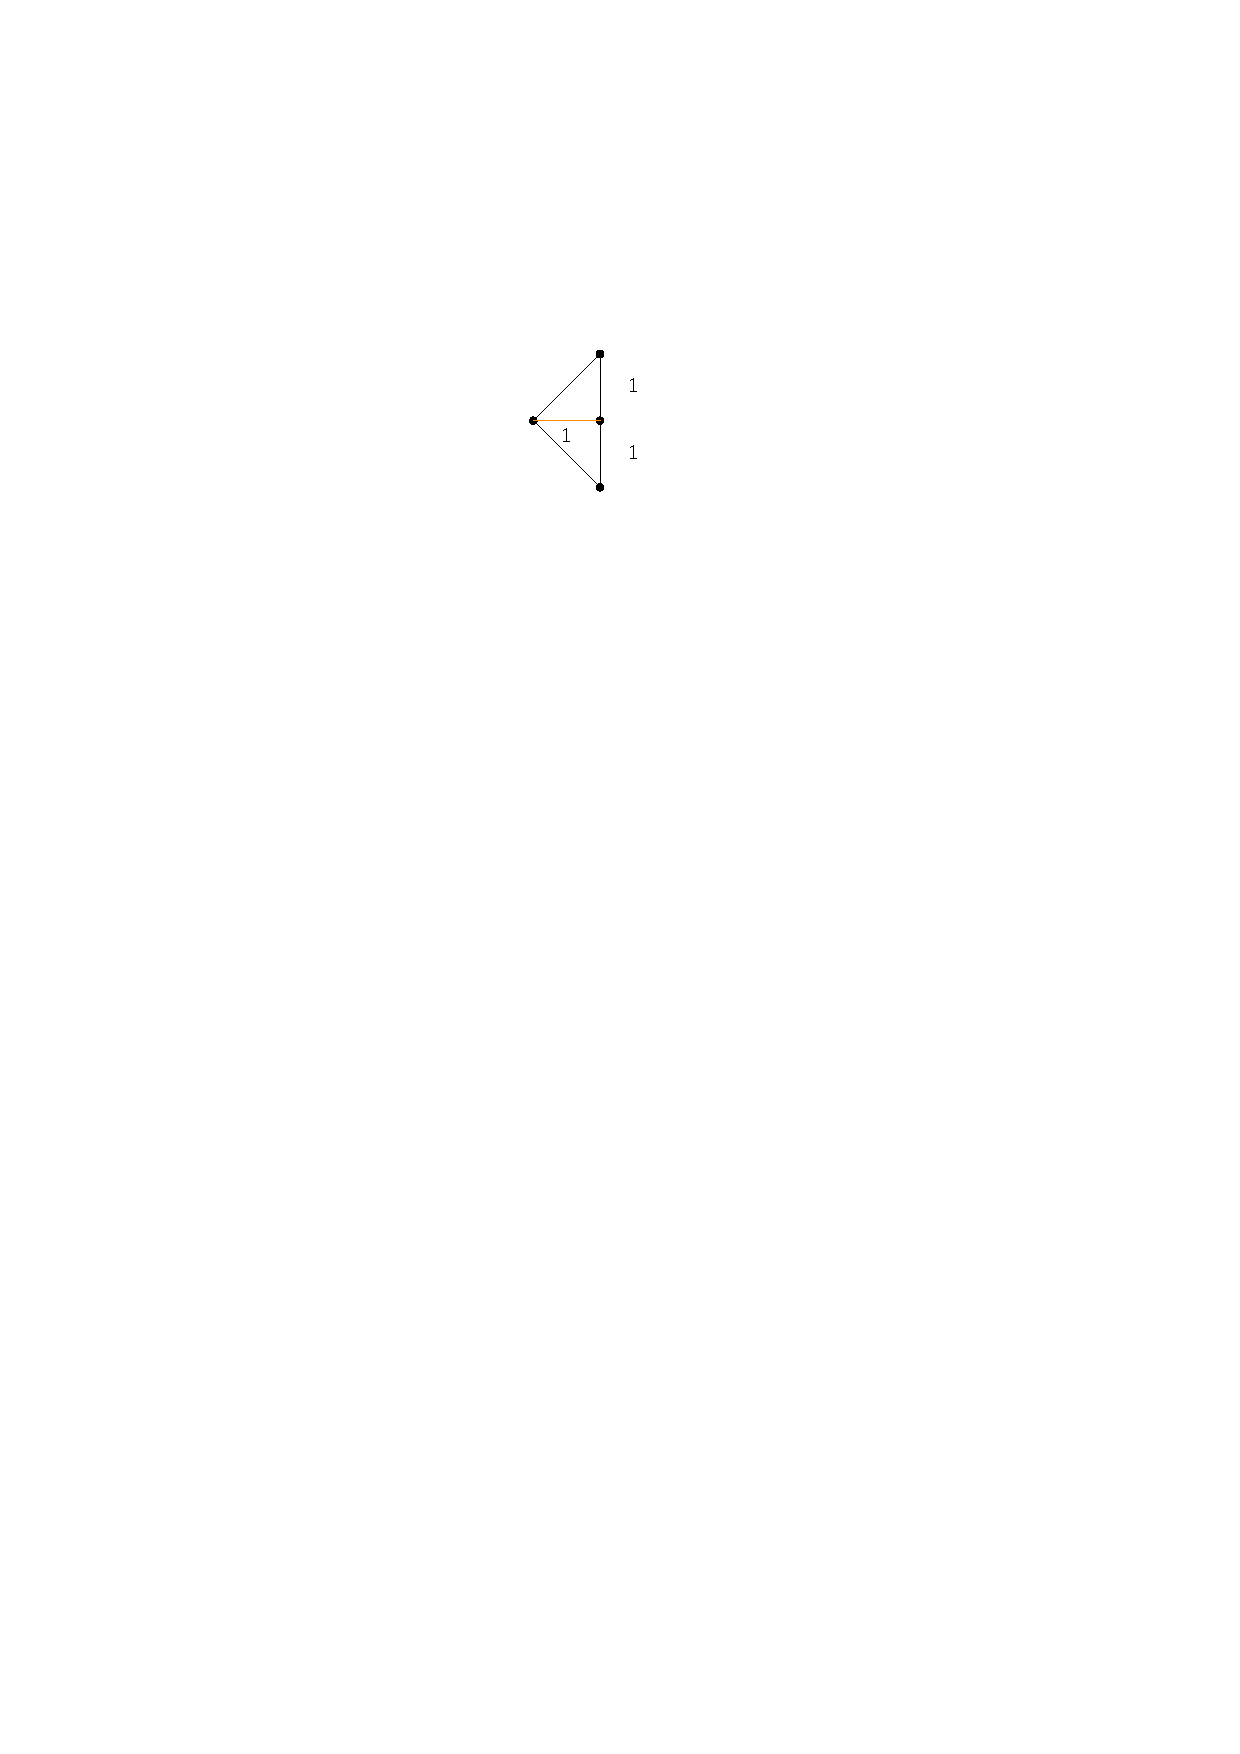
\includegraphics[width=0.7\textwidth,page=1]{drawings/maximal_planar.pdf}
	\end{subfigure}
\caption{An edge of \UL~(marked in orange), enclosed by two smallest-area triangles}\label{im:area_worst_case_straight-line}
\end{figure}
With a refinement in the first step, bend points are inserted into the adjacent triangles since their area consumption expands.


% Refinement

\subsection{Refinement step}
\begin{fact}\label{fact:area-expansion}
\end{fact}
Let $f$ be a face with an area consumption of $\mathcal{O}(a(k))$, $a(k)$ monotone increasing function and $k$ describing the granularity of the underlying grid. If the grid is refined by a factor of $c\cdot n$ for each dimension, then $f$ consumes area of $\mathcal{O}(c^2n^2 \cdot a(k))$.

\bigskip
So, by Fact \ref{fact:area-expansion}, the smallest possible area of a face now equals $\frac{1}{2}(cn)^2\UL^2$. Since every edge of unit length now is at least $c \cdot n$ long, the amount of bend points inside a face $f$ is bound by $\mathcal{O}((cn)^2)$. 
\begin{figure}[H]
	\centering
	\begin{subfigure}{0.3\linewidth}
		\centering
		\includegraphics[width=0.7\textwidth,page=2]{drawings/maximal_planar.pdf}
	\end{subfigure}
	\caption{The worst case from Figure \ref{im:area_worst_case_straight-line} after the refinement}\label{im:c-n_worst_case_straight-line}
\end{figure}
In the following sections, a straight-line drawing $\Gamma_G$ refined by a certain factor will be called $\Gamma'_G$, since the coordinates of the vertices changed. Although the shapes of the faces will stay the same, the area consumption is a different one.

% Supergraph extension

\subsection{Extending $G$ to a supergraph $G'$}
The supergraph is helpful for any transition of straight-line edge to a poly-line edge. It will describe where valid bend points lie. At first, the properties of maximal planar graphs is 

\begin{fact}\label{fact:even-subdivision}
\end{fact}
Let $f$ be a face of a drawing $\Gamma'_G$ with a constant amount of vertices defining it, inheriting area $\Theta(f(n))$. If $G$ is extended in a way that a new vertex, connected to all the vertices defining $f$, is placed inside $f$ so that $f$ is divided evenly, the resulting faces of the supergraph have still area $\Theta(f(n))$.
\begin{proof}
	Let $a$ be the area consumption of a face $f$, $a \in \Theta(f(n))$. Since the face is divided evenly by a constant amount $c$, every new face consumes at most $\frac{a}{c}+\varepsilon$ area and at least $\frac{a}{c}+\varepsilon'$ area $(\varepsilon,\varepsilon'>0)$. $\varepsilon, \varepsilon'$ describe the rounding error derived from the grid.
	\begin{align*}
		a \in \Theta(f(n)) \Rightarrow \frac{a}{c}+\varepsilon, \frac{a}{c}-\varepsilon' \in \Theta(f(n))
	\end{align*}
\end{proof}

\bigskip
So, if the grid is refined by $c\cdot n$, then, the face inheriting area $\frac{1}{2}(cn)^2\UL^2$ can be subdivided into three faces of roughly area $\frac{1}{6}(cn)^2\UL^2$ Since we are working on a grid with integers, there might be an approximation error which can be left out.

\begin{fact}\label{fact:maximal-planar-supergraph}
\end{fact}
Let $G$ be a maximal planar graph and $f$ a face of $G$. Extend $G$ to $G'$ by adding one vertex inside of $f$ and connecting to every vertex defining $f$. Then, $G'$ is maximal planar.
\begin{proof}
	If $f$ is an inner face, then it is a triangle with three vertices defining $f$. The vertex placed inside divides $f$ into three triangles, since it is connected to every of the three vertices defining $f$. $G'$ has now $v+1$ vertices, three more edges and one face is substituted with three smaller faces. Therefore, the amount of faces is increased by two and Eulers Formula holds.\\
	If $f$ is the outerface, then there are three vertices on the outerface, as well. Otherwise, there would be edges addable to $G$, and $G$ is not planar. The same holds for this case. 
\end{proof}

\bigskip
The intendation behind the vertex insertions is to evenly subdivide every face into three distinct new faces so every edge adjacent to two faces will have its own area reserved to be elongated in. This ensures the planarity of the output poly-line drawing naturally. The next Fact will answer the question where for each face, the vertices are inserted in practice.	

\begin{fact}\label{fact:centroid-point}
\end{fact}
Let $A,B,C$ be three points on the grid with their respective x and y coordinates, defining a triangle. Then, there exists a point $M$, called the centroid, which divides the triangle into three smaller triangles with roughly the same area usage, apart from a rounding error \cite{Centroid}. This point is defined as the arithmetic mean of $A,B,C$:
$$M\left(\frac{1}{3}(A_x + B_x + C_x), \frac{1}{3}(A_y+B_y+C_y)\right)$$

\bigskip

After the refinement and the graph extension, there are now sufficient bend points in reserved areas for every edge of $G$ to be elongated in availiable.

% Elongation

\subsection{Elongation step}
The general goal is to level all edge lengths occurring in $\Gamma'_G$. It is a question of how many bends are used in practice. The more bends are availiable, the more line segments can be inserted inside of a face. In the following section, the factor of refinement is specified along with a lower bound of the worst case scenario - the unit length edge with the smallest-area triangles possible attached to it.
\begin{fact}[Valid bend points]
\end{fact}
A grid point $b$ regarding a face $f$ is \textit{valid} iff it lies inside $f$ and the minimal distance to an edge defining $f$ lies in $(0,1]$.
\begin{fact}[Zig-zag elongation]\label{fact:poly-line-area-length}
\end{fact}
Let $A$ be a bounding box with area consumption $\mathcal{O}(a(k))$, where $k$ describes a granularity of the underlying grid. The height and the width of $A$ is described as $\mathcal{O}(h(k)), \mathcal{O}(w(k))$, respectively.  \\
A poly-line $p$ can be drawn inside $A$ with length $\mathcal{O}(a(k))$, using $\mathcal{O}(\min\{ h(k),w(k) \})$ bends.
\begin{proof}
	Let w.l.o.g. the height be larger than the width. The other case is valid analogously. The valid bend points are placed at the top and bottom row along the width at the bounding box. Start at one left corner of $A$ and draw a line segment along the height. For the following line segments, alternate with bends points between the top and bottom row until a right corner of $A$ is reached. The amount of bends are at most two times the width length. The length of the poly-line $p$ is therefore at most:
	\begin{align*}
		len(p) \leq (2\cdot w(k)+2) \cdot h(k) \in \mathcal{O}(w(k)h(k))
	\end{align*}
\end{proof}

\begin{lemma}\label{lemma:minimum-length}
\end{lemma}
When the grid is refined by a factor of $c\cdot n$ in each dimension, every edge of $\Gamma'_G$ can be elongated up to a length of $\Omega((c\cdot n)^2)$, using $O(c\cdot n)$ bends.
\begin{proof}
	Consider an edge $e$ of $\Gamma_G$ with \UL, enclosed by two smallest-area triangle faces. After the refinement and graph extension to $\Gamma'_{G'}$, the area consumption of the faces adjacent to $e$ values $\mathcal{O}((cn)^2)$[Fact \ref{fact:even-subdivision} and \ref{fact:area-expansion}]. Using all valid bend points in both faces adjacent to $e$, $e$ can be redrawn with $c\cdot n - 5$ line segments.
	
	\begin{figure}[H]
		\centering
		\begin{subfigure}{0.3\linewidth}
			\centering
			\includegraphics[width=0.7\textwidth,page=3]{drawings/maximal_planar.pdf}
		\end{subfigure}
		\caption{Using all valid bend points for line segment insertions}\label{im:all_valid_bend_points}
	\end{figure}
	
	$e$ is redrawn with a zig-zag elongation, using $2\cdot (cn-5)$ valid bend points. The new length of the sequence of line segments values at least:
	\begin{align}
		len(e) &\geq 3\cdot \left(2\cdot \sum_{i=1}^{\frac{cn-1}{3}-1}i + \sum_{i=1}^{\frac{cn-1}{3}-1}\sqrt{4i^2+1}\right)\\
		&> 3\cdot \left(2\cdot \sum_{i=1}^{\frac{cn-1}{3}-1}i + 2 \sum_{i=1}^{\frac{cn-1}{3}-1}i\right)\\
		&= 12 \cdot \sum_{i=1}^{\frac{cn-1}{3}-1}i\\
		&= \frac{2}{3}(cn)^2-\frac{10}{3}cn-\frac{4}{3}~~~\in \mathcal{O}((cn)^2)\label{eq:minimum-length-cn}
	\end{align}
\end{proof}
\bigskip

With this minimum length of $e$, drawn with as many line segments as possible, the following result can be achieved.
\begin{theorem}
	Let $\Gamma_G$ be given. If the drawing is refined by the factor of $n^2$, then there is sufficient area in $\Gamma'_G$ to elongate every edge so that the edge-length ratio is a constant.
\end{theorem}
\begin{proof}
	By equation \ref{eq:minimum-length-cn}, using $\mathcal{O}(n^2)$ bends, any edge can be elongated up to a length of $\mathcal{O}(n^4)$ while the length of the longest straight-line edge in an area of $\mathcal{O}(n^3)\times\mathcal{O}(n^3)$ lies in $\mathcal{O}(n^3)$.
\end{proof}

\bigskip
In practice, the longest edge of a straight-line drawing will not be altered in the transition from $\Gamma_G$ to $\Gamma'_G$.\\
So, by a refinement of $n^2$, it might be possible lengthen the shortest edge so that it is longer than the longest edge of $\Gamma'_G$. When the shortest edge can get longer than the longest one, then the same applies for every edge. But, this requires up to $2n^2$ bends per edge and is a bit over the top. In the next section, we will determine, that a linear amount of bends suffice so that the ratio is a constant.
%% Summary
\subsection{Using $n$ bends}

In the last section, it was shown that a refinement by a factor of $n^2$ suffices to level the lengths of all edges. In this section, the number of bends used per edge is fixed to $n$. At first, it is shown that the edge-length ratio will still be a constant when using $n+1$ line segments in order to draw an edge. Secondly, with help of the worst case example, a lower bound for the edge lengths is determined. Finally, the ratio will be investigated.
\begin{lemma}
\end{lemma}
With a refinement by a factor of $n^2$ and using $n$ bends and the supergraph extension as described above, the edge length ratio of the resulting drawing will lie in $\mathcal{O}(1)$.
\begin{proof}
	With $n$ valid bends, $n+1$ line segments are inserted into reserved faces of at least $\mathcal{O}(n^2)\times \mathcal{O}(n^2)$ area. Since the bend points are valid ones, they lie at the boundary of the corresponding faces. When inserting a line segment on opposing bend points, its length will lie in $\mathcal{O}(n^2)$, since it spans over one dimension of the face. $n+1$ line segments of such sort sum up to a total length of $\mathcal{O}(n^3)$. The length of the longest straight-line edge in a $\mathcal{O}(n^3)\times\mathcal{O}(n^3)$ drawing is also in $\mathcal{O}(n^3)$, therefore the ratio lies in $\mathcal{O}(1)$.
\end{proof}

\bigskip
Next, a lower bound of edge length is determined for a specific kind of face of $G$ - a triangle consisting of a horizontal line segment with length $w$ - also the edge to be elongated - a vertical line segment of height $h$ and the enclosing diagonal line segment. 
\begin{figure}[H]
	\centering
	\begin{subfigure}{0.4\linewidth}
		\centering
		\includegraphics[width=0.9\textwidth,page=4]{drawings/maximal_planar.pdf}
		\caption{}
	\end{subfigure}
	\begin{subfigure}{0.4\linewidth}
		\centering
		\includegraphics[width=0.9\textwidth,page=5]{drawings/maximal_planar.pdf}
		\caption{}
	\end{subfigure}
	\caption{A general width $w$ and height $h$, before (a) and after (b) grid refinement and graph extension}\label{im:h_greater_3w}
\end{figure}
When recalling the position of the centroid [Fact \ref{fact:centroid-point}], there are two cases of line segment insertions:\\
\underline{Case 1:} $h > 3w$\\
In this case, the height of the face created by the supergraph extension is larger than the length of the edge of interest with length $w$. 
\begin{figure}[H]
	\centering
	\begin{subfigure}{0.4\linewidth}
		\centering
		\includegraphics[width=0.9\textwidth,page=6]{drawings/maximal_planar.pdf}
	\end{subfigure}
	\caption{Inserting vertical line segments}\label{im:vertical_insertion}
\end{figure}
The line segments of the new polyline are inserted vertically, using valid bend points so that all the inserted line segments are as long as possible. 

\underline{Case 2:} $h \leq 3w$\\
In this case, the length of the original edge $e$ will at least as long as the new height to the inserted centroid $M$ of $G'$. So, the line segments will be placed horizontally, parallel to $e$. In order to preserve planarity, a bend point must be placed near the inserted vertex $M$. 
\begin{figure}[H]
	\centering
	\begin{subfigure}{0.4\linewidth}
		\centering
		\includegraphics[width=0.9\textwidth,page=7]{drawings/maximal_planar.pdf}
	\end{subfigure}
	\caption{Inserting horizontal line segments. The orange dotted bend points preserve planartiy}\label{im:horizontal_insertion}
\end{figure}
\begin{lemma}
\end{lemma}
For two positive integers $w,h>1$, it holds:
\begin{align*}
	\frac{hn^2-1}{wn^2-1}<h
\end{align*}
\begin{proof} The two cases of line segment insertions are covered with the following two cases:
	\begin{itemize}
		\item \underline{Case 1:} $h>w$\\
		\begin{align*}
			\frac{hn^2-1}{wn^2-1} < \frac{hn^2-n^2}{wn^2-n^2} = \frac{h-1}{w-1}< h
		\end{align*}
		\item \underline{Case 2:} $h \leq w$\\
		\begin{align*}
			\frac{hn^2-1}{wn^2-1} \leq \frac{hn^2}{wn^2} = \frac{h}{w} < h
		\end{align*}
	\end{itemize}
\end{proof}
\begin{lemma}
	When inserting up to $\frac{n}{2}$ line segments horizontally or vertically, depending on the height and the width of the face, the length of the resulting poly-line equals at least $n^3 - \mathcal{O}(n^2)$.
\end{lemma}

\begin{proof}
	\begin{itemize}
		\item Case 1: $h > 3w$\\		
		Let $f$ be a face in $\Gamma'_G$ defined by an horizontal edge $e = \overline{AB}$ with length $w' = w\cdot n^2$, w.l.o.g. a vertical line segment $\overline{BC}$ of length $h'=h\cdot n^2$, and the enclosing diagonal line segment. When the graph is extended to $G'$, the centroid is placed in $\Gamma'_{G'}$ at:
		\begin{align*}
			M\left(\frac{1}{3}(A_x+B_x+C_x) , \frac{1}{3}(A_y+B_y+C_y) \right)
		\end{align*}
		Since the x-coordinate of $B$ equals the one from $C$ and the y-coordinate of $A$ equals the one of $B$, it holds:
		\begin{align*}
			M\left(\frac{1}{3}A_x+\frac{2}{3}B_x , \frac{1}{3}C_y+\frac{2}{3}A_y \right)
		\end{align*}
		For further length calculations, the point $A$ is placed on the origin of the coordinate system. Then, the points are defined as follows:
		\begin{align*}
			A&(0,0)\\
			B&(w'-1,0)\\
			C&(w'-1,h'-1)\\
			M&\left(\frac{2}{3}(w'-1),\frac{1}{3}(h'-1)\right)
		\end{align*}
		\begin{figure}[H]
			\centering
			\begin{subfigure}{0.8\linewidth}
				\centering
				\includegraphics[width=0.9\textwidth,page=10]{drawings/maximal_planar.pdf}
			\end{subfigure}
			\caption{When $A$ is placed on the origin, this figure shows the positions and linear function descriptions of the faces}\label{im:coordinate_properties}
		\end{figure}
	
		When the y-coordinate of $M$ is greater than $w'$, then vertically inserted line segments will be longer than horizontally inserted ones. The elongation with $n$ bends and $\frac{n}{2}$ vertical line segments looks as follows:
		\begin{figure}[H]
			\centering
			\begin{subfigure}{0.6\linewidth}
				\centering
				\includegraphics[width=0.9\textwidth,page=8]{drawings/maximal_planar.pdf}
			\end{subfigure}
			\caption{Inserting vertical line segments in one face only}\label{im:vertical_one_face}
		\end{figure}
		And the lower bound of the total length can be estimated by the sum of the length of vertical line segments times two, since the diagonal line segments are at least as long as the vertical ones.
		\begin{align}
			len(e') &\geq \frac{1}{3}hn^2\cdot \frac{n}{2}-\left(1+\frac{1}{2}\left(\frac{h'-1}{w'-1}\right)\sum_{i=1}^{\left(\frac{n}{2}-1\right)\cdot\frac{2}{3}}i\right)-\left(\frac{h'-1}{w'-1}\sum_{i=1}^{\left(\frac{n}{2}-1\right)\cdot\frac{1}{3}}i\right)\label{eq:vertical}\\
			&+ \frac{1}{3}hn^2\left(\frac{n}{2}-1\right)-\frac{1}{2}h\frac{\left(\frac{n}{3}-\frac{2}{3}\right)\left(\frac{n}{3}+\frac{1}{3} \right)}{2}-h\frac{\left(\frac{n}{6}-\frac{1}{3}\right)\left(\frac{n}{6}+\frac{2}{3}\right)}{2}\label{eq:vertical-connectors}\\
			&=\frac{1}{3}hn^3-\left(\frac{4}{9}h-\frac{1}{2}w\right)n^2+\frac{1}{3}h
		\end{align}
	Since $h>3w$ and $h,w\geq1$, the length of the poly-line values at least $wn^3-\mathcal{O}(n^2)$ and the statement holds.
		\item Case 2: $h \leq 3w$
	In this case, the original straight line will be substituted with one horizontal line segment starting at $A$, ending in a bend point right before $B$. Furthermore, there will be a bend point right below $C$ in order to preserve planarity. The other horizontal line segments will be placed above the bottom one between $A$ and $B$. The line segments are shortened by $w$ from the right side and $2w$ from the left side, in total $3w$ per insertion. Since we only consider one face, the number of bend points and line segments is halved. 
	\begin{figure}[H]
		\centering
		\begin{subfigure}{0.6\linewidth}
			\centering
			\includegraphics[width=0.9\textwidth,page=9]{drawings/maximal_planar.pdf}
		\end{subfigure}
		\caption{Inserting $\frac{n}{4}$ horizontal line segments. The orange dotted bend point preserves planartiy}\label{im:horizontal_one_face}
	\end{figure}
	Then, the following lower bound for the length can be calculated:
	\begin{align}
		len(e') &\geq wn^2\cdot\left(\frac{n-2}{4}-3w\sum_{i = 1}^{\frac{n-2}{4}}i\right)\label{eq:horizontals}\\
		&+ wn^2\cdot \left(\frac{n-2}{4}-1\right)-3w\sum_{i=1}^{\frac{n-2}{4}-1}i\\
		&= \frac{1}{2}wn^3-\frac{35}{16}wn^2+\frac{3}{4}wn-\frac{3}{16}w
	\end{align}		
	This length is achieved by using the area of one adjacent face to $e$. However, this length is doubled when using both adjacent faces. The total length then values at least $wn^3-\mathcal{O}(n^2)$ and since  $w,h\geq1$, the statement holds.
	\end{itemize}
\end{proof}

\bigskip
\begin{lemma}
	The calculated minimum length also holds for any edge of $G$, regardless of the orientation of the adjacent faces.
\end{lemma}
\begin{proof}
	Since every face is a triangle, the defining line segments can always be described with help of a linear function $f(x)=mx+b$, as already done in Figure \ref{im:coordinate_properties}. Consider a valid bend point $K$. Then, the next valid point lies either above or below by one row, or left or right by one column. The actual position is determined by the slope of the linear function, describing the line segment next to $K$. This slope is a constant. So, by inserting a new horizontal line segment above or below a preexisting one occupying $K$, or by inserting a new vertical line segment left or right a preexisting one occupying $K$, the difference of length between those inserted line segments is a constant one. Therefore, the resulting length of the zig-zag line is of form $n^3-\mathcal{O}(n^2)$.
\end{proof}
\begin{theorem}\label{theorem:minimum-polyline-length}
\end{theorem}
In $\Gamma'_{G'}$, every edge of $G$ can be elongated to a poly-line with a length of at least $n^3 - \mathcal{O}(n^2)$, using $n$ bends.
\begin{proof}
	As a consequence of the refinement, every face $f$ inherits at least area of $\mathcal{O}(n^2)\times\mathcal{O}(n^2)$. When considering bend points only valid iff they lie on the boundary of $f$ and line segments must traverse the face, then there will be $n+1$ line segments inserted with a length of at least $n^2$, shortened by a linear amount in the worst case. This leads to $n$ line segments with length at least $n^2 - \mathcal{O}(n)$, summing up to a total length of at least $n^3-\mathcal{O}(n^2)$.
\end{proof}
\subsection{Summary}
The previous results can be summarized to the following theorems:
\begin{theorem}\label{theorem:max-planar-ratio1}
\end{theorem}
Let $G$ be a maximal planar graph, admitting a planar Schnyder straight-line grid drawing $\Gamma_G$ with a maximal area consumption of $(n-1)\times(n-1)$. Let $f(n)$ be a monotone function which describes the amount of bends per edge allowed. If $f(n) = n$, and the grid is refined by a factor of $n^2$, then $\Gamma_G$ can be altered to a poly-line drawing $\Omega_G$ such that the edge-length ratio lies in $\mathcal{O}(1)$ in area $\mathcal{O}(n^3) \times \mathcal{O}(n^3)$.
\begin{proof}
	Let $\Gamma_G$ be a Schnyder straight-line drawing of a maximal planar graph with $n$ vertices. Then, the edge-length ratio lies in $\mathcal{O}(n)$ since the length of the shortest edge values at least 1\UL~ and the length of the longest edge values at most $\sqrt{2}(n-1)$\\
	Refine the grid by a factor of $n^2$ in each dimension to obtain $\Gamma'_G$ in area $\mathcal{O}(n^3)\times \mathcal{O}(n^3)$. Then, by Fact \ref{fact:area-expansion}, every inner face consumes at least area of $\mathcal{O}(n^4)$.\\
	For each inner face $f$, a vertex is inserted and connected to each of the three vertices defining $f$. Mark the new vertices and edges. These new vertices extend $G$ to $G'$. $G'$ has $3n-6$ edges, there are 3 edges on the outerface and $3n-9$ inner edges. Every edge of $G$ is adjacent to two faces and enclosed by exactly four marked edges in $G'$. By Fact \ref{fact:even-subdivision}, the area enclosed by these marked edges is at least $\mathcal{O}(n^4)$ big and, by construction, this area is free in $\Gamma'_G$. By Fact \ref{fact:poly-line-length-equal-arbitrary-shape-area}, every edge of $G$ drawn in $\Gamma'_G$ can be elongated \grqq zig-zag wise\grqq~by a factor of $n$ bends used within the marked enclosing edges. For an edge of $G$ with length $\mathcal{O}(n^2)$ in $\Gamma_G'$, with $n$ bends the zig-zag elongation results in a length of $\mathcal{O}(n^3)$, by Theorem \ref{theorem:minimum-polyline-length} at least $n^3-\mathcal{O}(n^2)$ long. By leveling the length of all edges of $G$ to $\mathcal{O}(n^3)$ and deleting the edges and vertices of $G'\setminus G$ again, the result is a poly-line drawing $\Omega_G$ with an edge-length ratio of $\mathcal{O}(1)$ in area $n^2(n-1)\times n^2(n-1)$ and $n$ bends per edge.
\end{proof}
The following pseudocode sketches this drawing algorithm:\\
\begin{algorithm}[H]
	\KwIn{A Schnyder straight-line drawing $\Gamma_G$ in area up to $n-1\times n-1$}
	\KwOut{A poly-line drawing $\Omega_G$ with a minimized edge-length ratio}
	$\Gamma'_G \gets \Gamma_G.\texttt{RefineGrid}(n^2)$ \Comment{Grid refinement} \\
	$G'\gets G$\Comment{supergraph extension}\\
	\For{inner face $f$ of $G$}{
		$V(G') \gets V(G')\cup\{M_f\}$\Comment{$M_f$ subdivides $f$}\\
		$E(G') \gets E(G')\cup\{(M_f,A_f),(M_f,B_f),(M_f,C_f)\}$\Comment{$f$ defined by $A_f,B_f,C_f$}\\
		$\texttt{Pos}(M_f) = \frac{1}{3}\left(\texttt{Pos}(A_f)+\texttt{Pos}(B_f)+\texttt{Pos}(C_f)\right)$\\
		\texttt{DrawVertex}($M_f$)\\
		\texttt{MarkVertex}($M_f$)\\
		\texttt{DrawEdge}($\{(M_f,A_f),(M_f,B_f),(M_f,C_f)\}$)\\
		\texttt{MarkEdge}($\{(M_f,A_f),(M_f,B_f),(M_f,C_f)\}$)
	}

	$\texttt{float } l_{\max} \gets |\texttt{longestEdge}| $\\
	\For{edge $e$ in $E(G)$}{
		$\Gamma'_{G'}$\texttt{.EvalValidBendPoints($e$)}\Comment{Zig-zag elongation}\\
		\texttt{int bends}$\gets 0$\\
		\While{\texttt{bends}$<n-1 \wedge len(e)<l_{\max} $}{
			\texttt{bends}$\gets$\texttt{bends}$+2$\\
			\texttt{InsertLineSegment}$(e)$ \Comment{as long as possible}\\
			\texttt{DrawPolyLine}($e$)
		}
	}
	\For{$v \in V(G')$}{
		\If{$v$\texttt{.marked}}{$\Gamma'_{G'}$\texttt{.delete(v)}}
	}
	\For{$e \in E(G')$}{
	\If{$e$\texttt{.marked}}{$\Gamma'_{G'}$\texttt{.delete(e)}}
}
	\Return $\Gamma'_{G'}$	
	\caption{Modification of a straight-line drawing}
\end{algorithm}
\subsection{Runtime}
The above algorithm refines the grid by a factor of $n^2$, runtime $\mathcal{O}(n^2)$. Then, the subdivision takes place for every face, these are constant many operations for a linear amount of faces, ergo the runtime is $\mathcal{O}(n)$. The for loop in line 10 to 16: The validation of bend points may take $\mathcal{O}(n^3)$ since this is the area upper bound for the largest possible faces in a $\mathcal{O}(n^3)\times\mathcal{O}(n^3)$ drawing. And since there are a linear amount of edges (planar graph), the for loop may run in $\mathcal{O}(n^4)$ in the worst case. The deletion of the marked vertices and edges runs in linear time. The total runtime is therefore $\mathcal{O}(n^4)$.
\begin{theorem}
\end{theorem}
Every planar graph $G$ admits a poly-line drawing with an edge-length ratio of $\mathcal{O}(1)$ in area $\mathcal{O}(n^3)\times \mathcal{O}(n^3)$, allowing up to $n$ bends per edge.
\begin{proof}
	At first, add edges to $G$ so it is a maximal planar graph $G_{\max}$ and mark them. Then, draw $G_{\max}$ according to the proof of Theorem \ref{theorem:max-planar-ratio1}. The output is a poly-line grid drawing in area $\mathcal{O}(n^2)\times \mathcal{O}(n^2)$ with an edge-length ratio of $\mathcal{O}(1)$ and up to $\mathcal{O}(n)$ bends per edge. Afterwards, remove all marked edges from $G_{\max}$ to obtain $\Omega_G$.
\end{proof}

The following observation describes the behaviour of the ratio of large-scale graphs.
\begin{observation}
\end{observation}
Assuming, the base straight-line drawing $\Gamma_G$ is a Schnyder drawing, then with a refinement of $n^2$ and a usage of $n$ bends the edge-length ratio converges to $\sqrt{2}$ for $n \to \infty$.
\begin{proof}
	In a Schnyder straight-line drawing $\Gamma_G$, the area consumed values $n-1\times n-1$. The length of the longest edge values at most $\sqrt{2}(n-1) < \sqrt{2}n$. After the refinement by a factor of $n^2$, the longest edge values at most $\sqrt{2}n^3$. The ratio $r_G$ can then be expressed as:
	\begin{align*}
		r_G = \frac{\sqrt{2}n^3}{n^3-\mathcal{O}(n^2)} \underbrace{\rightarrow}_{n\to\infty} \sqrt{2}
	\end{align*}
\end{proof}
It is intuitive that for large scale graphs, the ratio might be better than for small-scale graphs. A refinement by a larger factor enables more bend points and alternations, leading to a better approximation for the edge-length levelling.
\begin{observation}
\end{observation}
Let $\Omega_G$ be a poly-line drawing of $G$ with a ratio of $r$, using $n$ bends. When the number ob bends is increased to $r\cdot n$, then the ratio tends to 1 for large-scale graphs.

\bigskip
The reason for this to happen is that every line-segment of the polyline has length at least $n^2 - \mathcal{O}(n)$. Using $r$ poly-lines, the length would be of form $r\cdot n^3 - \mathcal{O}(n^2)$. For large scale graphs, this might tend to 1. 

\subsection{An Example}\label{section:max_planar_example}
In order to see the whole postprocessing, the ratio of a straight-line drawing of the complete graph $K_4$ is minimized. The input is a straight-line drawing $\Gamma_{K_4}$ on a grid of size $3\times3$.
	\begin{figure}[H]
	\centering
	\begin{subfigure}{0.6\linewidth}
		\centering
		\includegraphics[width=0.9\textwidth,page=11]{drawings/maximal_planar.pdf}
	\end{subfigure}
	\caption{Input drawing of $K_4$ on a $3\times3$ grid}
\end{figure}
The ratio $r$ values $\sqrt{5}$, since the length of edge $(3,4)$ values 1 and the length of the edges $(1,4),(2,4)$ value $\sqrt{5}$.
Since $\mid V\mid = 4$, the grid is refined by $4\cdot 4$, resulting in a grid of size $48\times48$. The graph is extended, so that the area for edge elongations is defined.
	\begin{figure}[H]
	\centering
	\begin{subfigure}{0.6\linewidth}
		\centering
		\includegraphics[width=0.9\textwidth,page=12]{drawings/maximal_planar.pdf}
	\end{subfigure}
	\caption{Supergraph of $K_4$ on a $48\times48$ grid}
\end{figure}
Then, each edge is evaluated regarding its dashed cyan-colored bounding area and elongated with up to $n = 4$ bends.
	\begin{figure}[H]
	\centering
	\begin{subfigure}{0.6\linewidth}
		\centering
		\includegraphics[width=0.9\textwidth,page=13]{drawings/maximal_planar.pdf}
	\end{subfigure}
	\caption{Inserting up to 4 bends per edge for ratio minimization}
\end{figure}
	\begin{figure}[H]
	\centering
	\begin{subfigure}{0.6\linewidth}
		\centering
		\includegraphics[width=0.9\textwidth,page=14]{drawings/maximal_planar.pdf}
	\end{subfigure}
	\caption{$\Omega_{K_4}$}
\end{figure} 
For the edges $(1,2),(1,3),(2,3)$, the elongation was softened to approximate the longest edge. In order to demonstrate, what happens with maximum elongation, the previously shortest edge was elongated as long as possible. The calculated lengths are:
\begin{align}
	|(1,4)| = |(2,4)|&= 44,72\\
	|(1,2)| &= 44,39\\
	|(3,4)| &= 55,45\\
	|(1,3)| = |(2,3)| &= 43,56\\
	\Rightarrow r &= 1,28
\end{align}
The reason that $r$ is not quite optimal lies in the fact that the previously shortest edge became the longest edge. So, it seems that the algorithm requires further adjusting regarding the resulting edge lengths. The following alternative drawing inherits a nearly optimal ratio:
	\begin{figure}[H]
	\centering
	\begin{subfigure}{0.6\linewidth}
		\centering
		\includegraphics[width=0.9\textwidth,page=15]{drawings/maximal_planar.pdf}
	\end{subfigure}
	\caption{$\Omega'_{K_4}$}
\end{figure}
Here, $|(3,4)|=25,24$ and $r' = 1,04$. Nice.
\section{$k$-trees}
A new family of graphs is investigated for its edge-length ratio optimization on a fixed grid. A $k$-tree is an undirected graph which is incrementally created from a $K_{k+1}$ in a way that each added vertex has exactly $k$ neighbours such that those $k+1$ vertices form a clique. Following this definition, a $4$-tree is not planar since it starts with a $K_5$. Of interest is the 2-tree and the 3-tree. 
\subsection{2-trees}
For a 2-tree, each vertex is added to exactly two neighbours, forming a clique of size 3. Starting at a $K_3$, adding a vertex will create a new face since it forms a clique. For $n$ vertices, it holds: 
\begin{align}
	|E| = 2n-3 ~~~n\geq 3
\end{align}
\begin{proof}[Proof by induction]
	\underline{IA:} $K_3$ has three edges and three vertices, $3 = 2\cdot3-3 \checkmark$\\
	\underline{IV+IS:} Suppose, the statement is true for a 2-tree $T_i$ of size $i$. Adding a vertex to $T_i$ such that $T_{i+1}$ is still a 2-tree will connect the vertex $v_{i+1}$ to two neighbours in $T_i$, increasing the edge count by two.
	\begin{align*}
		|E_{T_{i+1}}| = |E_{T_i}| + 2 = 2\cdot i -3 + 2 = 2\cdot(i+1)-3
	\end{align*}
\end{proof}
Following Euler's Formula, the amount of faces for a 2-tree of size $n$ are:
\begin{align*}
	|F|+|V|-|E| &= 2\\
	|F| &= 2 + |E| - |V| = 2 + 2n-3 - n = n-1
\end{align*}
In a planar drawing, every edge is shared by exactly two faces. So when a vertex is added to a 2-tree drawing, there are at least two faces, where the vertex can be placed. In the figure below, an example is illustrated where a vertex can be placed in more than two faces.
\begin{figure}[H]
	\centering
	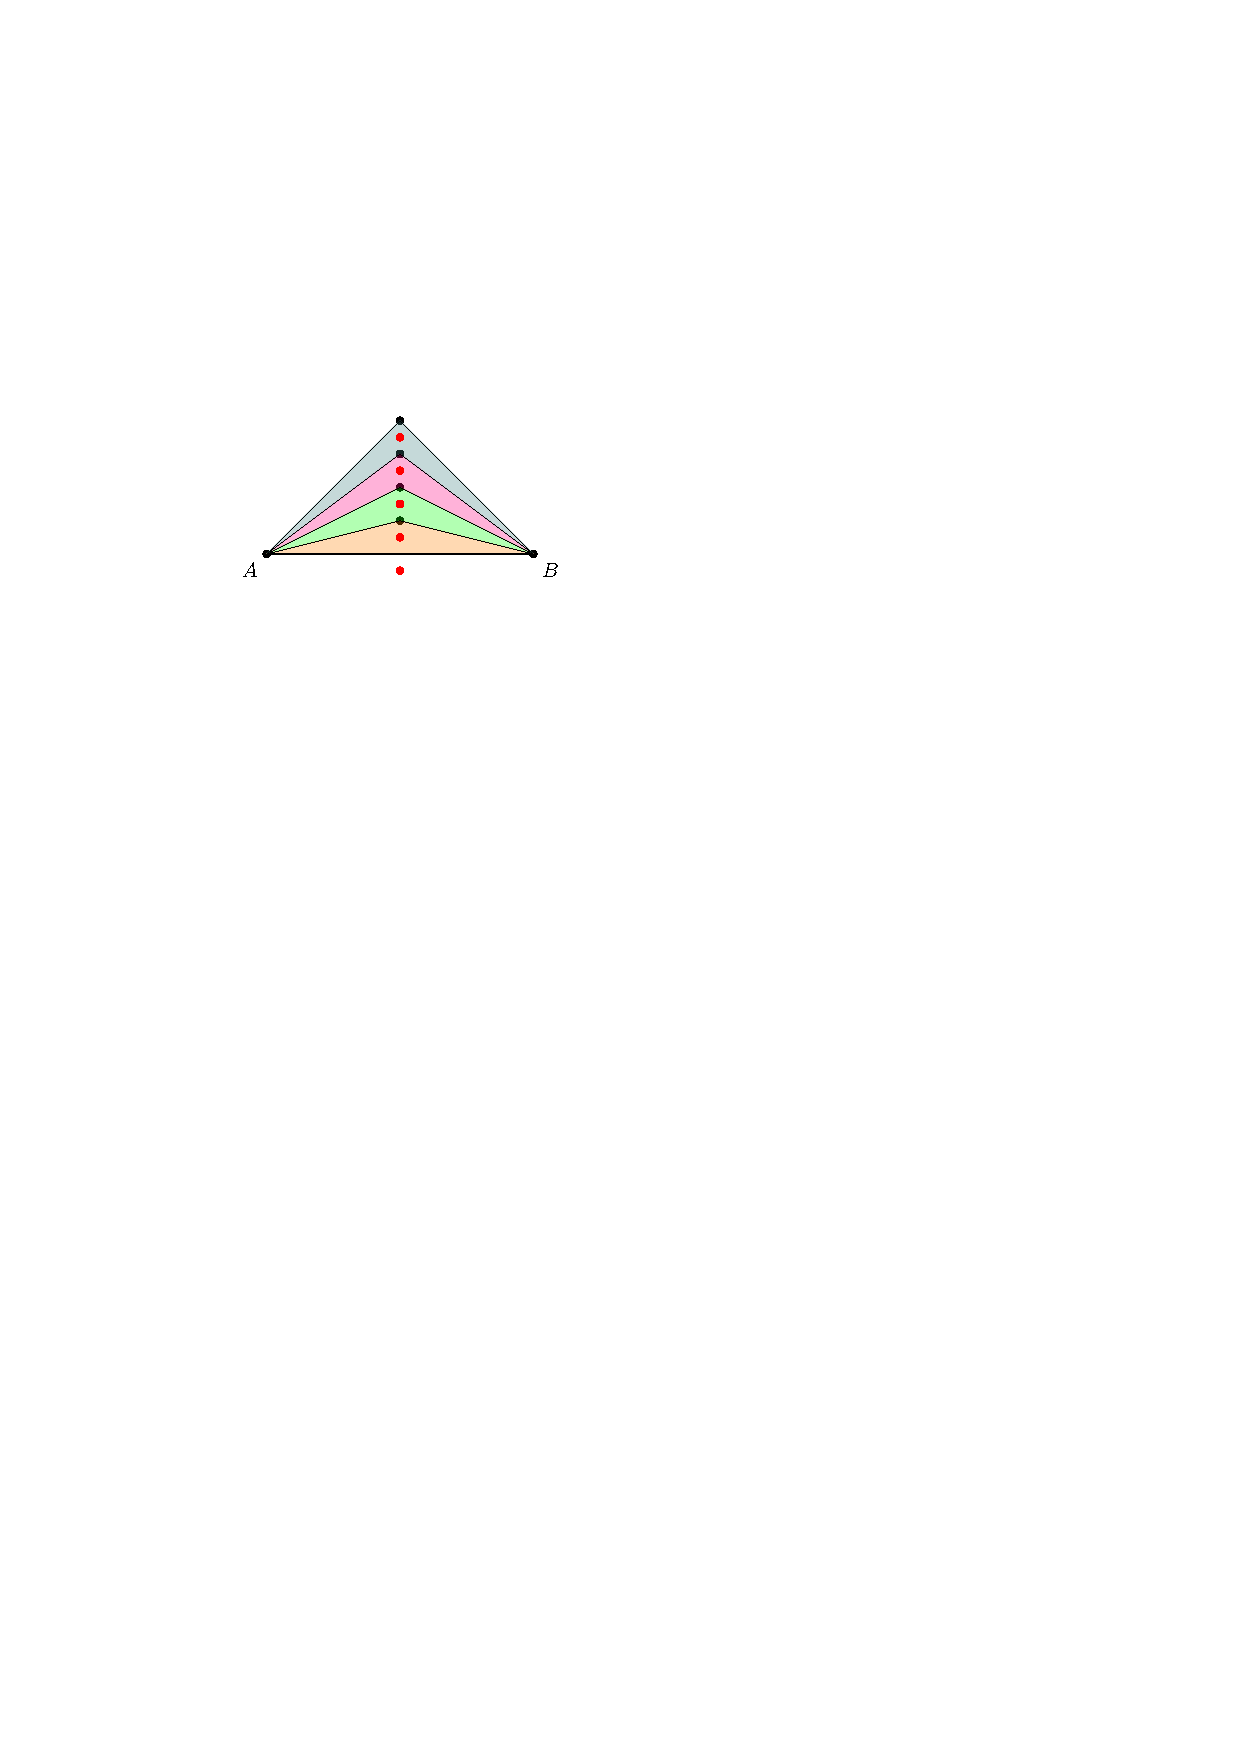
\includegraphics[width=.7\linewidth,page=1]{drawings/k-trees.pdf}
	\caption{In this drawing, a new vertex, forming a clique with A and B, could be placed in five faces, including the outerface, marked as red dot}\label{im:multiple-faces}
\end{figure}
The choice of face in which the vertex is drawn into might affect the edge-length ratio directly. One problem of a recursive drawing approach is that we do not know which problems might arise when deciding a face for a placement. So, we need a way to evaluate a suitable embedding for a given 2-tree graph.
\begin{lemma}[Expansion Lemma]
	If a graph G is $k$-connected and $G'$ is obtained by adding a vertex with at least $k$ neighbours in $G$, then $G'$ is k-connected.
\end{lemma}
\begin{proof}
	Since $G$ is $k$-connected, there are $k$ disjoint paths between every pair of vertices. Adding a vertex $v$ with $k$ neighbours will result in $k$ disjoint paths between $v$ and every other vertex of $G'$ since $G$ was already $k$-connected.
\end{proof}
\begin{theorem}
	A 2-tree is biconnected, but not necessarily triconnected.
\end{theorem}
\begin{proof}
	$K_3$ is biconnected since it is a cycle of size three. Since the 2-trees are recursively defined, adding subsequent vertices with exactly two neighbours will not harm the property of biconnectedness. In Figure \ref{im:multiple-faces}, this 2-tree serves as a counterexample for triconnectedness. A separation pair is $\{A,B\}$. Therefore, not every 2-tree is triconnected.
\end{proof}
By Spezielle Kapitel der Algorithmik Lecture about graph embeddings, the amount of embeddings for a biconnected graph is quite a lot. With $k$ parallel subgraphs, there are $k!$ permutations and every subgraph can be flipped additionally. Therefore, the amount of embeddings of biconnected graphs lies in $\mathcal{O}(n!2^n)$. Maybe, an SQPR Tree decomposition might help finding a \grqq good\grqq embedding regarding the edge-length ratio.\\
\subsubsection{First approach: Choice of vertex placement}
When adding a vertex, it will form a clique with pre-existing neighbours. This very edge is part of two faces. In this approach, the vertex added will be placed in the face with the larger area. The face will then be subdivided into two new faces. What happens, when the vertex is placed on the outerface?
\begin{lemma}
	Let $G$ be a drawing of a 2-tree and $v$ a vertex added to $G$ connecting to the neighbours defined by an edge on the outerface. Then, presuming, there is enough free area for it, $v$ can be placed on the outerface in a way that the edge-length ratio of $G'$ does increase derived by a rounding error of the grid.
\end{lemma}
\begin{proof}
	Let $l_{\max}$ be the length of the longest edge and $l_{\min}$ be the length of the shortest edge in the 2-tree $G$. We obtain $G'$ by adding a vertex $v$. If this vertex' neighbours are on the outerface and there is a free area box of size at least $l_{\min}\times l_{\min}$, then $v$ can be placed on the outerface with a distance between $l_{\min}$ and $l_{\max}$ to its neighbours and the edge-length ratio may increase when the edge-length ratio of $G$ was at 1. In this case, the placement of $v$ might not be possible to achieve edge lengths of $l_{\max}$. There will be a rounding error, depending on the granularity of the grid.
\end{proof}
So, placing vertices on the outerface will not increase the edge-length ratio significantly, presuming, there is enough free area to do so. This should work with any arbitrary number of bends per edge.\\
Now, we will investigate how the edge-length ratio behaves when a vertex is placed inside of a face. We will start with a drawing of a $K_3$, one bend allowed. We place a vertex inside of the $K_3$, creating new edges. Then, we will recursively add vertices to an edge which was created by the previous addition. The following algorithm will draw this special 2-tree:\\
\begin{algorithm}[H]
	\KwIn{$\Gamma$: Drawing of a $K_3$, $V_{\text{add}}=\{(v_i,e_i)\}$ vertices added and $|V_{\text{add}}| = m$}
	\KwOut{Drawing of a 2-tree with $m+3$ vertices}
	InsertVertex($v$,$e$) $= \{$\\
	~~~~Choose the face adjacent to $e$ with the larger area except for the outerface\\
	~~~~Place the vertex and the edges with bends in this face in a way that the face is subdivided evenly in area\\
	$\}$
	\While{$V_{\text{add}}\neq \emptyset$}{
		\For{$i \in [1..|V_{\text{add}}| = m]$}{
		\If{$e_i$.drawnIn$\Gamma$}{
		InsertVertex($v_i$,$e_i$)\\
		$V_{\text{add}} \gets V_{\text{add}}\setminus\{(v_i,e_i)\}$
		}	
	}
}
\end{algorithm}
In the special case described above, the set $V_{\text{add}}$ is initialized as follows:
\begin{align*}
	(v_1,e_1)\in V_{\text{add}}~~~e_1\text{ arbitrary edge of }K_3\\
	(v_i,e_i)\in V_{\text{add}}~~~e_i\text{ edge created by inserting }v_{i-1}\\	
\end{align*}
In this special case, the runtime of the algorithm above is in linear time. It is of interest, how the edge-length ratio will behave. In the following figures, vertex and bend placements were done intuitively.
\begin{figure}[H]
	\centering
	\begin{subfigure}{0.4\textwidth}
		\centering
		\includegraphics[width=.7\linewidth,page=2]{drawings/k-trees.pdf}
		\caption{Start with a $K_3$}
	\end{subfigure}
\begin{subfigure}{0.4\textwidth}
	\centering
	\includegraphics[width=.7\linewidth,page=3]{drawings/k-trees.pdf}
	\caption{Insert $v_1$ to neighbours $A$ and $B$}
\end{subfigure}
\begin{subfigure}{0.4\textwidth}
	\centering
	\includegraphics[width=.7\linewidth,page=4]{drawings/k-trees.pdf}
	\caption{Insert $v_2$ to neighbours $A$ and $v_1$}
\end{subfigure}
\begin{subfigure}{0.4\textwidth}
	\centering
	\includegraphics[width=.7\linewidth,page=5]{drawings/k-trees.pdf}
	\caption{Insert $v_3$ to neighbours $v_1$ and $v_2$}
\end{subfigure}
\begin{subfigure}{0.4\textwidth}
\centering
\includegraphics[width=.7\linewidth,page=6]{drawings/k-trees.pdf}
\caption{Insert $v_4$ to neighbours $v_2$ and $v_3$}
\end{subfigure}
\begin{subfigure}{0.4\textwidth}
	\centering
	\includegraphics[width=.7\linewidth,page=7]{drawings/k-trees.pdf}
	\caption{Insert $v_5$ to neighbours $v_3$ and $v_4$}
\end{subfigure}

\begin{subfigure}{0.4\textwidth}
	\centering
	\includegraphics[width=.7\linewidth,page=8]{drawings/k-trees.pdf}
	\caption{Insert $v_6$ to neighbours $v_4$ and $v_5$}
\end{subfigure}
\caption{Example of a nested drawing with one bend per edge, edge-length ratio in $\mathcal{O}(2^n)$}
\end{figure}
The edge-length ratio worsens with every inserted vertex. The shortest edge created by the $i$-th insertion has $\approx \frac{3}{4}$ length of the previous shortest edge. Therefore, the edge-length ratio in the $i$-th insertion values $\left(\frac{4}{3}\right)^i$. For $n$ vertices, the edge-length ratio of a 2-tree lies in $\mathcal{O}(2^n)$ in the worst case with this approach and one bend allowed per edge. Note, that it was not allowed to draw on the outerface.
\begin{observation}
	If it is allowed to draw on the outerface, then the above example can be drawn with an edge-length ratio of approximately 1. The edge-length ratio does not rise for an added vertex significantly, when allowing two bends per edge.
\end{observation}
\begin{figure}[H]

		\centering
		\includegraphics[width=.4\linewidth,page=14]{drawings/k-trees.pdf}
		\caption{Insert $v_i$ to neighbours $v_{i-1}$ and $v_{i-2}$, outerface allowed}

\end{figure}
There are edges which worsen the edge-length ratio, since a bend placement is not possible to maintain the uniform polyline edge-length without violating the planarity. In this example, this refers to the edges $(v_1,v_3)$, $(v_3,v_5)$ and $(v_4,v_6)$. Point of interest is, when does the special case of inserting a vertex in a face apply? In the following alternation of the example, we can observe where this case applies.
\begin{figure}[H]
	\centering
	\begin{subfigure}{0.7\textwidth}
		\centering
		\includegraphics[width=.7\linewidth,page=15]{drawings/k-trees.pdf}
		\caption{Vertex $r$ added to $A$ and $v_1$ on the outerface, since the area is bigger than the face defined by $A,B,v_1$}
	\end{subfigure}
\begin{subfigure}{0.7\textwidth}
	\centering
	\includegraphics[width=.7\linewidth,page=16]{drawings/k-trees.pdf}
	\caption{Then, vertex $v_2$ is added to $v_1$ and $A$ as before. The face defined by vertices $A,B,v_1$ is larger than the other face created by the insertion of $r$}
\end{subfigure}

\begin{subfigure}{0.7\textwidth}
	\centering
	\includegraphics[width=.7\linewidth,page=17]{drawings/k-trees.pdf}
	\caption{With every insertion of vertex $v_i$, the edge-length ratio roughly doubles}
\end{subfigure}
\caption{Example where the special case applies}
\label{im:v16r-rfirst}
\end{figure}
\begin{observation}
	When drawing $v_2$ first on the outerface, the edge-length ratio does not worsen as drastically as in the figure above.
\end{observation}
\begin{figure}[H]
	\centering
	\includegraphics[width=.4\linewidth,page=18]{drawings/k-trees.pdf}
	\caption{The same graph, but with a different ordering of edges around $v_1$  (two bends allowed)}
	\label{im:ABCv16+r}
\end{figure}
The edge $(A,v_1)$ formed two cliques, one with $r$ and one with $v_2$. More cliques are adjacent to the clique formed with $v_2$ in comparison to $r$. It was a good decision to place $v_2$ on the outerface since the outerface will provide the area to draw the remaining cliques without increasing the edge-length ratio significantly. Some sort of ordering will be helpful to evaluate the properties of a drawing.\bigskip
\begin{definition}
	For a given 2-tree $G$, the edge-clique graph $EC_G$ is defined as follows:
\end{definition}
	\begin{itemize}
	\item $V(EC_G)$ consists of the edge set of $G$, namely $E(G)$ and the clique set of $G$, namely $C(G)$.
	\item For $e = (a,b) \in  E(EC_G)$, either $a \in E_G$ and $b\in C_G$ or vice versa. If $a,b$ are both in $E(G)$ or $C(G)$, then $(a,b)\notin E(EC_G)$.
	\item For a clique vertex, there are exactly three edges vertices adjacent.
	\item For an edge vertex, there are arbitrary many clique vertices adjacent.
\end{itemize}
\begin{lemma}
	For a connected 2-tree $G$, the corresponding edge clique graph $EC_G$ is a tree.
\end{lemma}
\begin{proof}
	Suppose, that $EC_G$ is not connected. Then, there are at least two vertices which are not connected by a path. This means that there is an edge or a clique in $G$ which is not connected to the rest of the graph. But $G$ is connected. Therefore, $EC_G$ is connected.\\
	Suppose, there was a cycle in $EC_G$. Then, the cycle is of even length because of the edge restriction in $EC_G$. Consider a clique vertex $c$ of the cycle. It has two paths to another clique vertex of the cycle. Since every edge and clique of $G$ is represented once in $EC_G$, this destroys the 2-tree property.
\end{proof}
The following drawing represents a $EC_G$ for the example above in Figure \ref{im:ABCv16+r}.
\begin{figure}[H]
	\centering
	\includegraphics[width=.4\linewidth,page=19]{drawings/k-trees.pdf}
	\caption{$EC_G$ for the example of Figure \ref{im:ABCv16+r}}
\end{figure}
\begin{lemma}
	Let $p$ be a path of $EC_G$, beginning at an edge vertex and ending in an edge vertex. Then, drawing the corresponding cliques only will have an edge-length ratio of $\mathcal{O}(1)$.
\end{lemma}
\begin{proof}
	Start by drawing the starting edge. Then, draw the corresponding clique. Since $p$ is a path, the next clique will be drawn on the outerface. As we have seen before, adding a vertex to the outerface does not increase the edge-length ratio significantly.
\end{proof}
\begin{observation}
	Let $p_{\max}$ be the longest path in $EC_G$. Let $\Gamma$ be the drawing of $G$ where the longest path is drawn at first. Let $\Gamma'$ be an alternate drawing where a shorter path was drawn at first. Then, it is possible that the edge-length ratio of $\Gamma'$ is worse than the ratio of $\Gamma$.
\end{observation}
Recall the example above and the drawing resulting in Figure \ref{im:v16r-rfirst}. Drawing a shorter path in the $EC_G$ first resulted in a drawing where the longer path was not drawn on the outerface. This increased the edge-length ratio significantly.
\subsection{Previous results regarding series-parallel graphs}
There are several results for small planar drawings of outerplanar and series-parallel graphs. It was shown that:
\begin{itemize}
	\item Every series-parallel graph has a visibility representation with $\mathcal{O}(n^{\frac{3}{2}})$ area
	\item Every series-parallel graph has a visibility representation with $\mathcal{O}(\Delta n\log n)$ area, where $\Delta$ is the maximum degree of the graph
	\item It was reproven that every outerplanar graph is series-parallel, therefore these results also apply for outerplanar graphs [\cite{DBLP:journals/dcg/Biedl11}: Page 2,3]
\end{itemize}
Visibility respresentations and orthogonal drawings can be converted to polyline drawings. The following relationships hold for drawing models:
\begin{description}
	\item[Visibility Representation] Vertices are boxes, edges are horizontal or vertical line segnemts. In a 1-directional visibility representation all edges are vertical line segments.
	\item[Orthogonal Box-Drawing] Vertices are axis-aligned boxes (possibly degenerated to a line segment or point) and edges are sequences of contiguous horizontal or vertical line segments. A 1-directional visibility representation is also automatically an orthogonal box-drawing. In a flat orthogonal box drawing, every vertex is a vertical line segment.
	\item[Poly-line drawing] Vertices are points, edges are sequences of contiguous straight-line segments. A transition point between two straight-line segments is called a bend. A poly-line drawing can be obtained by modifying an orthogonal box drawing in a way such that a vertex is reassigned to a point inside of the prior box and the incident edges are rerouted to this very point. Also, empty grid lines are added until every edge has length at least 2. The area consumption is asymptotically the same since the width and height is doubled at most.
	[\cite{DBLP:journals/dcg/Biedl11}: Page 5,6]
\end{description}
Since visibility representations and orthogonal box drawings can be converted to polyline drawings with asymptotically the same area, the upper bounds given for the visibility representation also hold for poly-line drawings.
\subsection{The drawing algorithm for a maximal series-parallel graph}
A 2-terminal series parallel graph with terminals $s,t$ is defined recursively.
\begin{itemize}
	\item An edge $(s,t)$ is a 2-terminal SP graph
	\item If $G_i, i=1,2$ is a 2-terminal SP graph with $s_i, t_i$, then a serial composition with $s = s_1$, $t=t_2$ and $s_2 = t_1$ is a 2-terminal SP graph
	\item If $G_i,i=1,...,k$ is a 2-terminal SP graph, then, the parallel composition unifies $s_i$ to $s$ and $t_i$ to $t$ and the resulting graph is a 2-terminal SP graph
\end{itemize}
A series-parallel graph is a graph for which every biconnected component is a 2-terminal series-parallel graph. It is maximal if no edge can be added while maintaining a simple SP graph.
The drawing algorithm which proves the area bounds creates a visibility representation of a given maximal series-parallel graph and is also defined recursively based on 2-terminal SP graphs. The maximum height of the drawing is given by a recursive formula, depending of the heights of the subgraphs. [\cite{DBLP:journals/dcg/Biedl11}: Page 6 to 11]
Concerning the edge-length ratio, the longest edge might depend on the height of the drawing while the shortest edge might be of unit length.
\begin{description}
	\item[Invariant] Vertex $s$ contains the upper right corner of the bounding box, while vertex $t$ contains the lower right corner of the bounding box. The boxes for $s$ and $t$ can be stretched to the whole width of the drawing 
	\item[Base case] the base case is the edge $(s,t)$. Simply put $s$ over $t$ and the invariant holds
	\item[Height] The height of a drawing, denoted by $h$, can be increased preserving the invariant
	\item[Inductive step] This step is for $m>1$ edges and holds two major cases: a parallel composition and a serial composition. If the composition is a parallel one, then the recursive drawings of the $k$ parallel subgraphs will be of a serial composition and vice versa.
	\begin{itemize}
		\item During the parallel composition, $2\leq k$ subgraphs will first be ordered in their number of edges $(m_i \leq m_{i-1}, i \in[1..k])$ and then recursively drawn. The subgraphs are drawn in serial since the original step is the parallel case. The heights of the subgraph drawings are adjusted and unified with a terminal $s$ and $t$ on top and bottom of the bounding box.
		\item For the serial composition, two subgraphs $H_a, H_b$ with terminals  $s,x$ and $x,t$ are recursively drawn (in parallel). Note, that $x,t$ is an edge of $H_b$ since the original graph is a maximal series-parallel one. There are two outcomes of serial placement. Either, the boxes for $x$ and $t$ share the same row on the bottom of the bounding box, being connected horizontally, or $x$ lies in an interior row and is connected to $t$ vertically
	\end{itemize}
	\item[Output] The resulting drawing is a flat orthogonal box drawing. There are no additional columns for the vertices, every vertex contains an incident vertical edge in the base case. Since no bend is created at any time, the box drawing is in fact a flat visibility representation. It was shown that the height of the drawing is bound by $\mathcal{O}(\sqrt{n})$ and there are maximal as many columns as there are edges. The resulting drawing is in area $\mathcal{O(n^{\frac{3}{2}})}$.
	\item[Runtime] Since in this recursive algorithm every edge is touched exactly once, the total runtime lies in $\mathcal{O}(m+n)$.
\end{description}
\subsection{Edge-length ratio of a maximal series-parallel graph}
In the resulting flat orthogonal drawing without any bends / visibility representation with $\mathcal{O}(n)$ width and $\mathcal{O}(\sqrt{n})$ height, the longest edge lies in $\mathcal{O}(n)$ since edges are horizontal or vertical line segments. The shortest edge is in $\mathcal{O}(1)$ in the base case.
\subsubsection{From a flat orthogonal drawing to a polyline drawing}
To transfer a flat orthogonal drawing to a polyline drawing, empty grid lines are inserted until every edge length is at of least two. For a box of a vertex $v$, replaced the box by an arbitrary grid point and insert a bend for each edge connected to $v$ for rerouting. For each vertex, a bend might be inserted, resulting in a polyline drawing with up to two bends per edge.
\begin{lemma}
	Every maximal series-parallel graph admits a polyline drawing with two bends per edge and an edge-length ratio of $\mathcal{O}(n + \sqrt{n}) = \mathcal{O}(n)$.
\end{lemma}
\begin{proof}
	In the transition, every box of vertex in the orthogonal box drawing is substituted with a dot on the grid, therefore two bends per edge. A vertex box has width at most $\mathcal{O}(n)$, like the total width. The longest vertical edge lies in $\mathcal{O}(\sqrt{n})$, is horizontally rerouted with a line segment in $\mathcal{O}(n)$. The shortest edge stays in $\mathcal{O}(1)$, therefore the total edge-length ratio lies in $\mathcal{O}(n)$.
\end{proof}
\subsection{Next steps}
\begin{description}
	\item[Improve the worst case result] If this approach is a correct one, find a way to improve the exponential worst case of the edge-length. 
	\item[Investigate 3-trees] Since 3-trees are triconnected, there is one embedding disregarding flip. How does the edge-length ratio behave? Which face would be suitable to put on the outerface?
\end{description}

% \subsection{3-trees}
\section{Other Results}

\subsection{$k$-nary trees}
\begin{lemma}The depth of a complete $k$-nary tree $d$ values $\left\lfloor\log_k((k-1)n)\right\rfloor$
\end{lemma}
\begin{proof}
	\begin{align}
		n &= \sum_{i=0}^{d}k^i = \frac{k^{d+1}-1}{k-1}\\
		\Leftrightarrow d &= \log_k((k-1)n+1)-1 = \left\lfloor\log_k((k-1)n)\right\rfloor
	\end{align}
\end{proof}

\begin{theorem}
	Every $k$-nary tree admits a polyline drawing with a nearly optimal ratio, apart from a rounding error $\varepsilon$ on area $\mathcal{O}(n^2\log n)$, allowing one bend per edge.
\end{theorem}
\begin{proof}
	Generally, the reulting drawing will be constructed from top to bottom. The root vertex lies on top, the leaves lie on the bottom. Let $l := k^d +1$. From the root vertex, place one vertex $k^d $ \UL~to the left and one unit down. Place another child $k^d$ \UL~to the right and one unit down. For the remaining $k-2$ children, place bends inbetween those outer children equidistantly. Connect the two children and the bend points with the root with a line segment. There, the rounding error takes effect and is bound by $1$. Place the remaining children below the respective bends so that the sum of the line segment equals $l$, apart from the rounding error. Between two children, there are $\frac{2k^d}{k-1}-2$ free columns for the remaining drawing.\\
	Further iterate over the depth. For depth $i$, place the outermost children $k^{d-(i-1)}$ aside and one unit down and the $k-2$ bend points in between equidistantly. From the preceding depth, there are $\frac{2k^{d-(i-2)}}{k-1}-2$ free columns between two children of depth $i$ placed next to each other. Since $\frac{k^{d-(i-1)}}{k-1}\leq \frac{k^{d-(i-2)}}{k-1}$, the area for depth $i+1$ is guaranteed.\\
	The total width of the drawing is bound by $2\cdot \sum_{i=0}^{d}k^i \in \mathcal{O}(n)$, and the total height is bound by $d\cdot l = d\cdot (k^d+1) \in \mathcal{O}(n \log n)$. Every edge has length of approximately $l$, apart from a rounding error derived by the diagonals with one bend per edge and the total area consumption values $\mathcal{O}(n^2\log n)$.
\end{proof}
\begin{figure}[H]
	\centering
	\begin{subfigure}{0.8\linewidth}
		\centering
		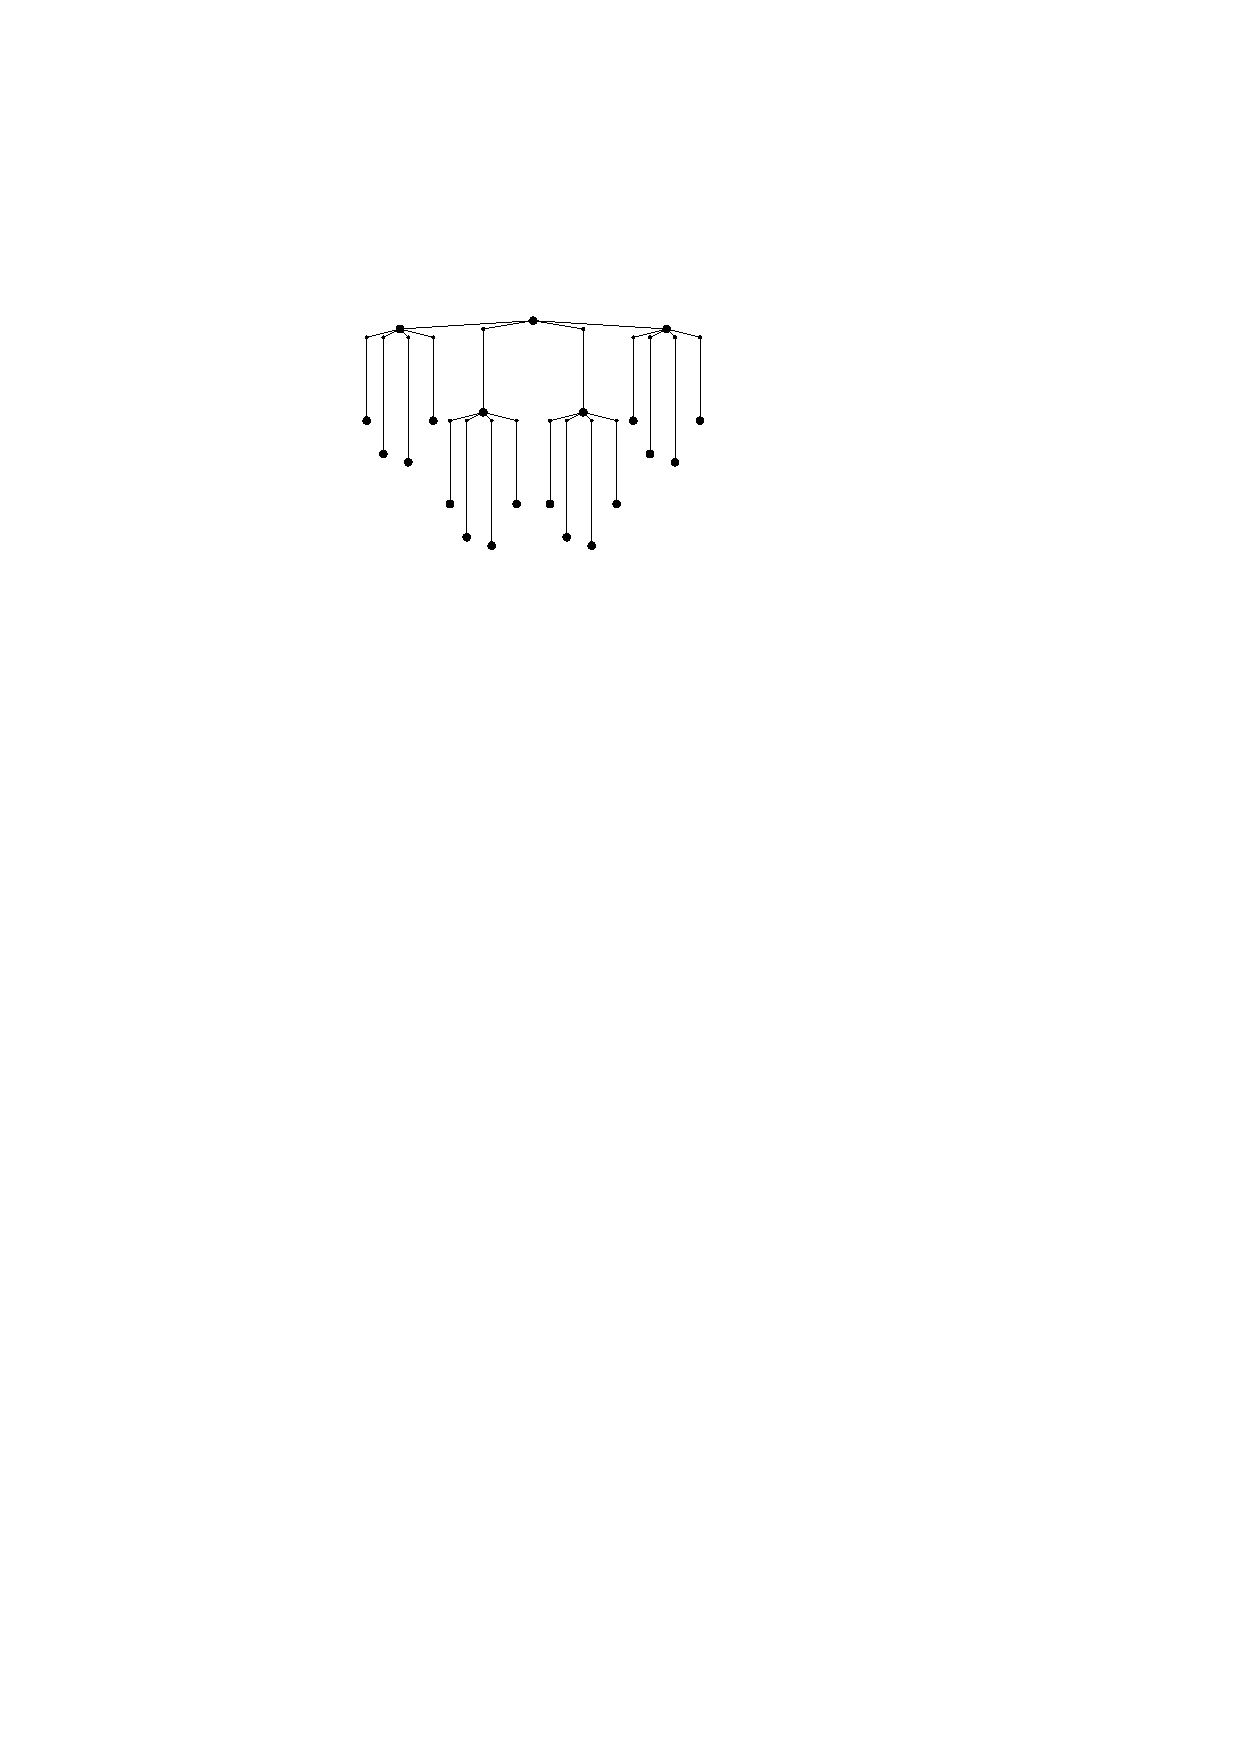
\includegraphics[width=\textwidth,page=1]{drawings/4-ary_tree.pdf}
	\end{subfigure}
	\caption{Complete 4-ary tree with depth 2}\label{im:4-ary_d=2}
\end{figure}
\begin{figure}[H]
	\centering
	\begin{subfigure}{0.8\linewidth}
		\centering
		\includegraphics[width=\textwidth,page=2]{drawings/4-ary_tree.pdf}
	\end{subfigure}
	\caption{Complete 3-ary tree with depth 3}\label{im:4-ary_d=2}
\end{figure}
\subsection{Certain family of 3-trees}\label{section:3-tree-family}
Recall a $k$-tree, recursively defined. A 3-tree starts with a $K_4$ and every vertex inserted is connected to exactly three neighbours, creating a 4-clique.
\begin{theorem}
	There exists a family of 3-trees which obtain a polyline drawing with a constant edge-length ratio, allowing one bend per edge on area $\mathcal{O}(n^2)$.
\end{theorem}
\begin{proof}
	Let $G$ be a graph consisting of $\frac{n}{3}$ socalled \grqq nested\grqq~triangles, meaning that every triangle either encloses or is enclosed by another triangle.  Let $t_1$ be the outermost triangle and $t_{i+1}$ inside $t_i,i=1,...,\frac{n}{3}$. The vertices defining $t_i$ are called $A_i,B_i,C_i$. For the orientation, $A_i$ will be on the bottom left corner, $B_i$ on the bottom right corner and $C_i$ on the top corner. The edges between the triangles are defined as:
	\begin{align}
		&(A_i,A_{i+1}),(A_i,B_{i+1}),(A_i,C_{i+1})\\
		&(B_i,B_{i+1})\\
		&(C_i,C_{i+1}),(C_i,B_{i+1})
	\end{align}
		\begin{figure}[H]
	\centering
	\begin{subfigure}{0.8\linewidth}
		\centering
		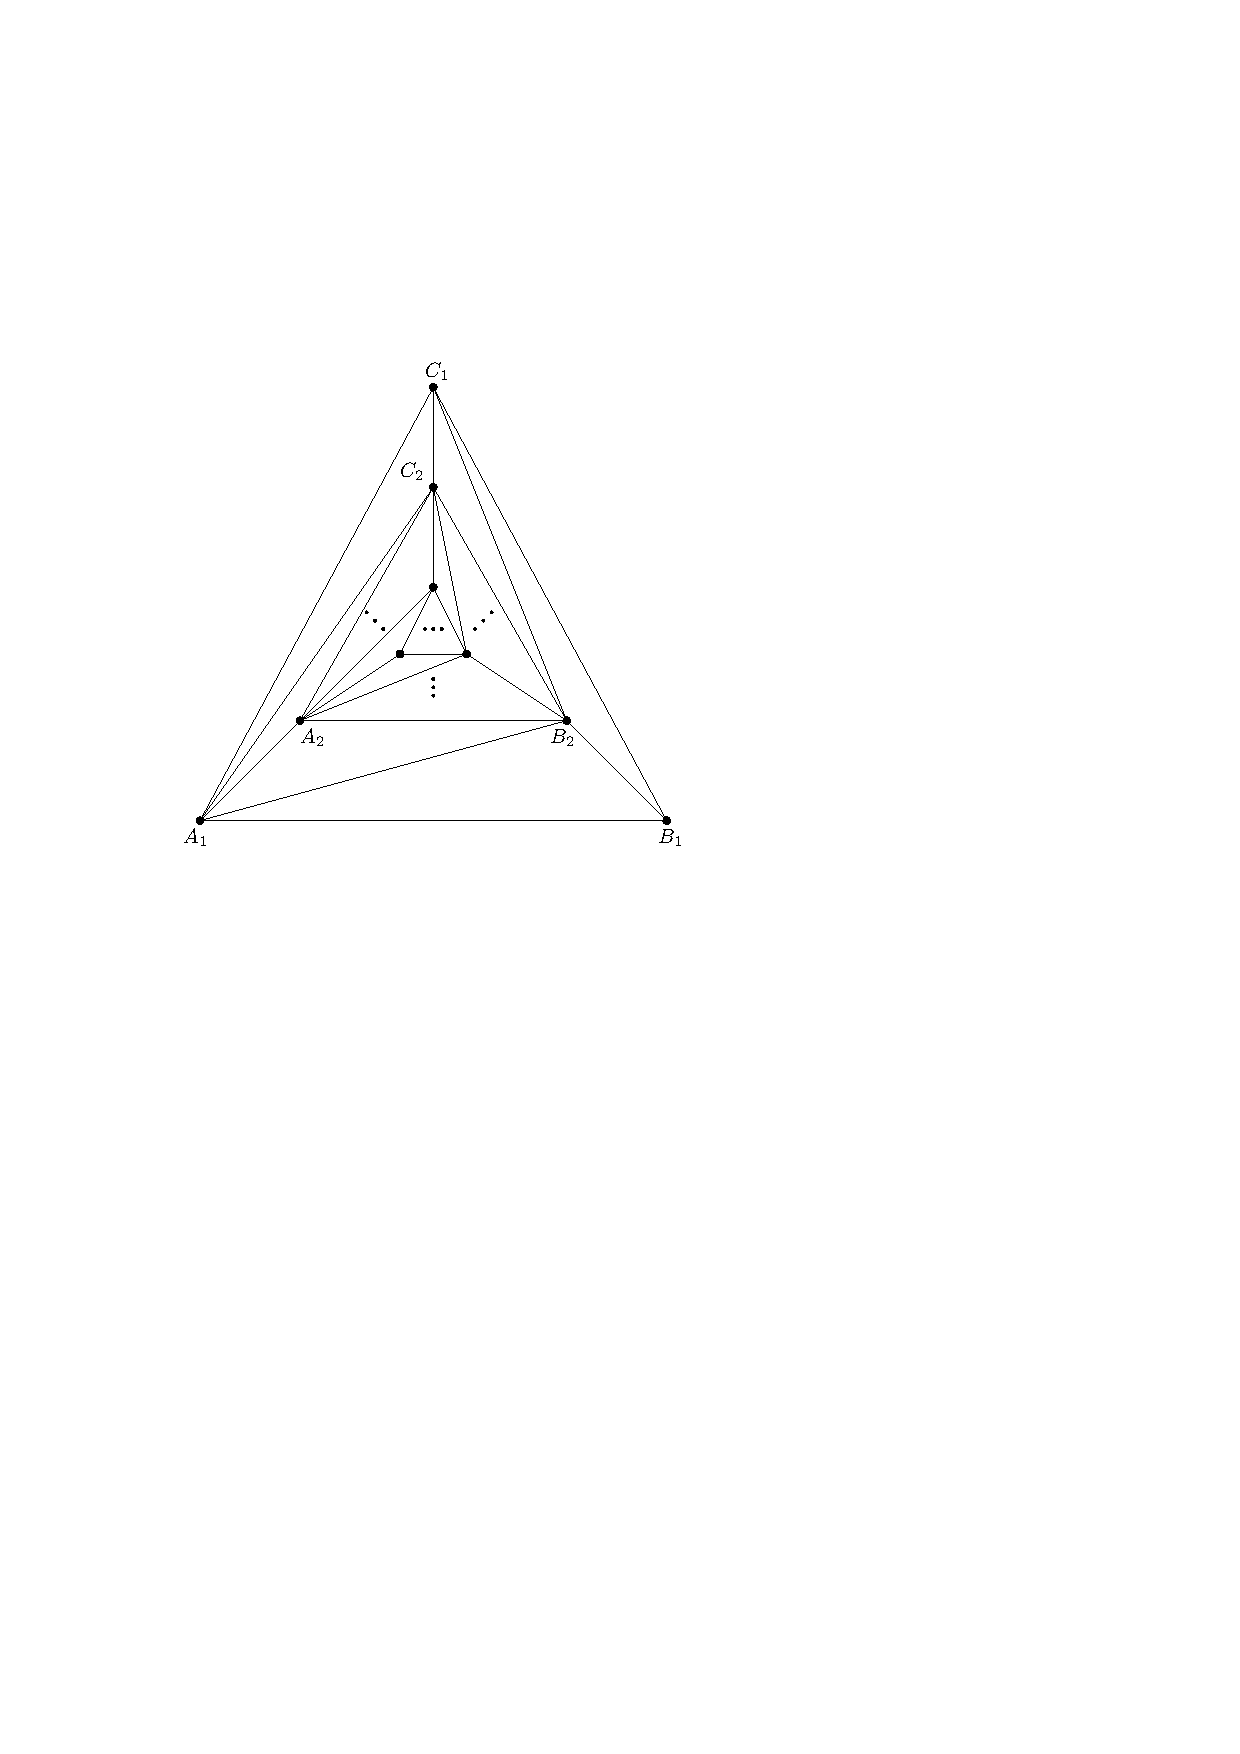
\includegraphics[width=\textwidth,page=1]{drawings/3-tree.pdf}
	\end{subfigure}
	\caption{3-tree with nested triangles}\label{im:3trees-straight-line}
\end{figure}
	The connections between the triangles $t_i,t_{i+1}$ fulfill the 3-tree property. (\cite{DBLP:journals/jgaa/MondalNRA11}, Lemma 12, Page 23).
	At first, draw the triangles with a spacing of three between two consecutive triangles. This ensures two rows or columns of availiable bend points inbetween. Placing bends will lengthen the connections between two successive triangles. The bend points are placed as illustrated in the following figure:
		\begin{figure}[H]
		\centering
		\begin{subfigure}{0.8\linewidth}
			\centering
			\includegraphics[width=\textwidth,page=2]{drawings/3-tree.pdf}
		\end{subfigure}
		\caption{Polyline drawing scheme with one bend per edge}\label{im:3trees-drawing}
	\end{figure}	
	Then, the length of every connecting edge between $t_i$ and $t_{i+1}$ is greater than the shortest edge of $t_{i+1}$. The total shortest edge lies in $t_{\frac{n}{3}}$. The total longest edge lies in $t_1$. Let the length of the edges of $t_{\frac{n}{3}}$ value $n$. Then, the length of the edges of $t_1$ value $n+2\cdot 3\left(\frac{n}{3}-1\right) = 3n-6$. The ratio is bound by 3, the spacing value. The output is a polyline drawing with one bend per edge on a grid of area $(3n-6)\times(3n-6)$.
\end{proof}
\subsection{Outerplanar graphs}
Outerplanar graphs are a family of series-parallel graphs. The result of 2-trees can be applied directly to outerplanar graphs. The following theorem describes the edge-length ratio in a poly-line drawing while maintaining that every vertex is placed on the outerface.
\begin{theorem}
	Every outerplanar graph $G$ obtains a poly-line drawing with an edge-length ratio of $\mathcal{O}(1)$ with up to four bends per edge in $\mathcal{O}(n^2)$ area.
\end{theorem}
\begin{proof}
	Since outerplanar graphs are series-parallel graphs, this proof is similar to the proof of Theorem \ref{theorem:2-tree_result}. By Biedl, it was proven, that only the base case, the parallel case and the serial case S1 and S2a take place (\cite{DBLP:journals/dcg/Biedl11}, Page 15). All the cases guarantee that the vertices lie on the outer face.
	\begin{figure}[H]
		\centering
		\begin{subfigure}{0.8\linewidth}
			\centering
			
\includegraphics[width=0.8\textwidth,page=14]{drawings/2-trees.pdf}
		\end{subfigure}
		\caption{Case S2a is the only case for outerplanar graphs}\label{im:outerplanar}
	\end{figure}
	With the modification used in Theorem \ref{theorem:2-tree_result}, the height can be bound by:
	\begin{align}
		h_{mod}(m)\leq 3\log m + 2 + l_{\min} + 1\leq 3(\log 2 +1)+3\cdot \log n + n \in \mathcal{O}(n)
	\end{align}
	The longest edge can occur in case S2a, with two bends in the box drawing. In the polyline drawing, two additional bends are introduced for vertex $v,t$. Therefore, the longest edge is bound by:
	\begin{align}
		l_{\max}\leq 2(w_{mod}(m)+h_{mod}(m))= 6\cdot \log 2 +6\log n + 14n - 2
	\end{align}
	Then, it holds for the ratio:
	\begin{align}r \leq \frac{20n}{n} = 20 \in \mathcal{O}(1)
	\end{align}
\end{proof}
\section{Future Work}
\subsection{Tweaking the postprocessing algorithm}
A refinement of $n^2$ and using $\frac{n}{2}$ line segments as long as possible successfully overcomes the hurdle of leveling the edge lengths. But, as seen in the example in Section \ref{section:max_planar_example}, the lengths of the elongated edges might get longer than the original longest edge. The trend is that almost all edges will be longer than the longest edge. This is not desirable, since this worsens the ratio again by re-allocating the longest edge of the modified drawing. So, the question is how to adjust to the original longest edge without getting longer. Either, by not using the longest possible line segment insertions by default, or by using less bends in total. Maybe, a refinement by $o(n^2)$ suffices, for example a refinement by $n$ or $n\log n$. It does prove that the area suffices for every edge to be elongated in and shows a first approach. But, considering the trend of getting the edges too long, the postprocessing algorithm presented in this report is not applicable in this state.
\subsection{Further minimizations}
We observed that a linear amount of bends is mandatory for the edge-length ratio to be bound by a constant. It would be of interest to further minimize either the number of bends without losing any upper bounds or the area the whole drawing takes place in. This would be achieved by further investigating and gauging the postprocessing algorithm. 
\subsection{New drawing algorithm approach} 
Take a look at the certain 3-tree family presented in Section \ref{section:3-tree-family}. On one hand, the postprocessing algorithm proved that a refinement of at least $n$ and zig-zag elongations result in a constant ratio. But, this family of 3-trees (maximal planar) are drawable with a constant ratio and still remain in area $\mathcal{O}(n^2)$. This exclusive nestedness of this graph family might give a hint that a certain property of graphs determine the upper bound for the area while guaranteeing a constant ratio. This might be something interesting to further investigate.
\subsection{Implementation}
When the postprocessing algorithm is remastered, an implementation of this algorithm will be of interest. The readability of a drawing will suffice with a high amount of zig-zag elongations. But, when the number of bends or the length of the inserted line segments is minimized further, the readability will be an aspect of interest when the implementation is there.
\printbibliography
\end{document}
